%=======================================================================
%  esreg -- Endogenous switching regression with heterogeneous selection
%  on gains: assumptions, tests, and estimation. Skeleton, September 2026
%  A. Araar, Universite Laval / PEP
%  Companions: selection_on_gains.tex (paper A), msat_note.tex (paper B)
%=======================================================================
\documentclass[11pt,a4paper]{article}
\usepackage[margin=2.5cm]{geometry}
\usepackage{amsmath,amssymb,amsthm}
\usepackage{booktabs}
\usepackage{array}
\newcolumntype{L}[1]{>{\raggedright\arraybackslash}p{#1}}
\usepackage{xcolor}
\usepackage{graphicx}
\usepackage{listings}
\usepackage{tikz}
\usetikzlibrary{positioning}
\usepackage[round,authoryear]{natbib}
\usepackage[colorlinks=true,linkcolor=blue!55!black,citecolor=blue!45!black,urlcolor=blue!55!black]{hyperref}

\lstset{basicstyle=\ttfamily\small,columns=fullflexible,keepspaces=true,
        frame=single,framesep=4pt,rulecolor=\color{gray!50},breaklines=true,
        xleftmargin=6pt,xrightmargin=6pt}

\newcommand{\todo}[1]{\par\smallskip\noindent%
  \textcolor{red!70!black}{\small$\blacktriangleright$ \textsf{TODO:} #1}\par\smallskip}

\theoremstyle{plain}
\newtheorem{proposition}{Proposition}
\newtheorem{lemma}{Lemma}
\newtheorem{corollary}{Corollary}
\theoremstyle{definition}
\newtheorem{assumption}{Assumption}
\newtheorem{definition}{Definition}
\theoremstyle{remark}
\newtheorem{remark}{Remark}

\newcommand{\E}{\mathbb{E}}
\newcommand{\Cov}{\operatorname{Cov}}
\newcommand{\Var}{\operatorname{Var}}
\newcommand{\Corr}{\operatorname{Corr}}
\newcommand{\ATT}{\mathrm{ATT}}
\newcommand{\ATU}{\mathrm{ATU}}
\newcommand{\ATE}{\mathrm{ATE}}
\newcommand{\MTE}{\mathrm{MTE}}
\newcommand{\PRTE}{\mathrm{PRTE}}
\newcommand{\1}{\mathbf{1}}
\newcommand{\cmd}[1]{\texttt{#1}}

\newcommand{\kX}{\kappa(x)}

\title{\bf Endogenous Switching Regression with Heterogeneous Selection on Gains:\\
Assumptions, Tests, and Estimation}
\author{Abdelkrim Araar\\
\small Universit\'e Laval and Partnership for Economic Policy (PEP)}
\date{October 2026\\
\small Software: \texttt{esreg} 1.0.0\quad Zenodo: \url{https://doi.org/10.5281/zenodo.22717029}}

\begin{document}
\maketitle

\begin{abstract}
\noindent
The endogenous switching regression is the one workhorse model in which
selection on gains---the covariance $\kappa$ between the gain from
treatment and the unobservable that drives participation---is a free
parameter rather than an assumption. This paper asks under what
conditions the selection equation identifies $\kappa$, how each
condition can be checked, and which estimation route to take when a
condition fails. It orders the assumptions by what they cost: a normal
single-index selection equation, a linear conditional mean of the regime
errors given the participation error, and trivariate normality, together
with the exclusion, sufficiency and variation conditions on the
instruments. It then gives one test per assumption, all borne by the
selection equation: a link test and a probit-versus-FIML contrast for the
index, a test of index sufficiency for the instruments, diagnostics of
strength and support, a Wald test of constant $\kappa$ in the covariates,
a Hausman contrast with an influence-function covariance and Hermite
controls that separate a failure of trivariate normality from a failure
of the linear conditional mean, and a pseudo-difference-in-differences
on the index whose within-group contrasts read selection on gains off a
two-by-two table with almost no model. Estimation proceeds by tiers,
removing one assumption at a time: full-information maximum likelihood
with heterogeneous variances and correlations, a two-step estimator
with the exact variance of the whole procedure from stacked moments, the
same two-step augmented by Hermite terms when the conditional mean is
not linear, and a semiparametric marginal treatment effect on the score. The model
extends to $\kappa(x)$, a selection on gains that varies with the
covariates. Monte Carlo experiments give the tests their size and show
that each rejects what it is built to reject; the manual example of
Stata's \cmd{etregress} shows the reading changing the conclusion. The
Stata command \cmd{esreg} and its family of post-estimation commands
implement the whole, with survey weights, clusters and the survey
design; they are validated value for value against a Python reference
implementation and against \cmd{etregress}, \cmd{movestay} and \cmd{msat},
and their standard errors against brute-force influence functions and a
Monte Carlo.

\medskip\noindent
\textbf{Keywords:} endogenous switching regression, selection on gains,
marginal treatment effect, specification tests, Stata.\\
\textbf{JEL:} C21, C31, C52, C87.
\end{abstract}

%=======================================================================
\section{Introduction}\label{sec:intro}
%=======================================================================
A program that people join voluntarily is evaluated on the outcomes
of those who joined and of those who did not, and the difference
between the two groups mixes the effect of the program with the reasons
for joining. When those reasons are related to what the program would
do for each person---when the ones who join are the ones who gain
most, or least---the average effect on the treated, the average effect
on the untreated and the average effect in the population are three
different numbers, and a policy that extends the program to
non-participants yields the second, not the first. \citet{araar2026sog}
called this selection on gains, defined it as the covariance $\kappa$
between the gain from treatment and the unobservable that drives
participation, and showed that among the models practitioners use, the
endogenous switching regression (ESR) of \citet{roy1951},
\citet{heckman1978} and \citet{maddala1983} is the only one in which
$\kappa$ is a parameter to estimate rather than a restriction to
impose: matching and inverse-probability weighting set it to zero
conditionally on covariates, difference-in-differences differences it
away under a common trend, the single-equation treatment regression
forces one correlation on both regimes. The price of that freedom is a
set of assumptions, and the ESR has a reputation for fragility that
comes from them: it is said to rest on trivariate normality and on
exclusion restrictions that the data cannot test, and to be identified
by functional form when the instrument is weak.

This paper takes the reputation apart. Its starting point is the
observation that the fragilities of the ESR are properties of its
selection equation, not of the joint normality of its errors taken as a
block. Three things are asked of the selection equation: an argument
(the exclusion restriction, and the less discussed requirement that the
instruments act on the regime errors only through the participation
index, which the paper calls index sufficiency), a form (a normal
single index, whose Mills ratios are the control functions of both
estimation routes), and variation (enough movement of the index within
covariate cells for the control function to be told apart from the
covariates). The joint law of the regime errors given the participation
error is asked for only by the likelihood, in two pieces that can be
separated: a linear conditional mean, which the two-step route also
needs, and normality of the regime errors around it, which it does not.
Ordering the assumptions this way makes each one testable with the
material the selection equation provides, and it makes the choice of an
estimation route a consequence of the tests rather than a matter of
taste.

The paper makes three contributions. The first is a set of tests, one
per assumption, all computed from the probit index and the two regime
regressions. For the form of the selection equation, a link test and
a contrast between the probit and the likelihood estimates of the
selection coefficients, which is what trivariate normality imposes on
the selection equation. For index sufficiency, the addition of the
excluded instruments but one to the regime regressions beside the Mills
ratio, whose coefficients are zero under the null and whose sign reads
a direct effect of the instrument on the outcome. For the joint law, a
Hausman contrast between the likelihood and the two-step estimates with
a covariance built from the influence functions of the two
estimators---positive semi-definite by construction, valid under the
alternative---and Hermite controls beside the Mills ratio that detect a
nonlinear conditional mean; the two tests separate the two failures,
which matters because they call for different remedies. For the
strength and support of the instrument, diagnostics that say how much of
the identification rests on the curvature of the Mills ratio. And a
model-light test of selection on gains itself: a
pseudo-difference-in-differences on strata of the participation index,
whose two within-group contrasts have the signs of $\rho_1\sigma_1$
and $\rho_0\sigma_0$ under the linear conditional mean alone, and
whose ratio to the $X$-adjusted contrasts of the Mills ratios is a
consistent estimator of $\kappa$ that never uses the joint law.

The second contribution is $\kappa(x)$, a selection on gains that
varies with the covariates: $\rho_j\sigma_j(x)=W(x)'\theta_j$ in the
two-step route, where the Mills ratio interacted with $W$ is the
regressor and $\kappa(x)=W(x)'(\theta_1-\theta_0)$ is identified under
the same conditions as the constant model plus a rank condition; and
heterogeneous $\ln\sigma_j$ and $\operatorname{atanh}\rho_j$ in the
likelihood. A program whose selection on gains is stronger among the
educated, or among the poor, is then a testable hypothesis, and the
marginal treatment effect becomes a surface in $(x,p)$. The third
contribution is the estimation by tiers and its implementation: the
likelihood with analytic scores, the two-step with the exact variance
of the whole procedure from the stacked moment conditions of the probit
and the two regressions---the variance that \cmd{msat}
\citep{araar2026msat} obtained by bootstrap and that \cmd{etregress}
provides only for its constrained model---, the same two-step augmented
by Hermite terms when the conditional mean bends, the effects with the
influence function of the whole procedure, and the semiparametric
marginal treatment effect on the score by percentile-weights regression
\citep{araar2026pwr}, the tier that keeps only the single index. The
Stata command \cmd{esreg} and its post-estimation family
(\cmd{esrdiag}, \cmd{esrtest}, \cmd{esrcurve}, \cmd{esrmte},
\cmd{esrreport}) implement all of it, with factor variables, survey
weights, clusters and survey designs; every printed number is checked
against a Python reference implementation written first, and every
standard error against a brute force.

The paper sits next to three literatures. The marginal treatment effect
of \citet{heckman2005} is the object the semiparametric tier estimates
and the object the parametric line summarizes; the ESR is the index
model in which the MTE is a line, and $\kappa$ is its slope. The
discrete-instrument literature of \citet{brinch2017} and the bounds of
\citet{mogstad2018} address the same identification problem from the
other side, asking what a discrete instrument can deliver without a
parametric line; the paper's diagnostics of variation and support say
where that question bites, and the manual example of
Section~\ref{sec:emp}, with a single indicator instrument, shows the
semiparametric tier failing for exactly that reason. And the Stata
implementations---\cmd{movestay} \citep{lokshin2004}, \cmd{msat}
\citep{araar2026msat}, and the official \cmd{etregress} with the
\cmd{poutcomes} option, which fits the same likelihood
\citep{statacorp2025}---estimate the model but do not test it; the paper's
Section~\ref{sec:cmd} sets the four side by side.

Section~\ref{sec:model} presents the model, $\kappa(x)$, and the
assumptions ordered by cost. Section~\ref{sec:ident} states what each
route identifies and what happens when index sufficiency fails.
Section~\ref{sec:tests} develops the tests. Section~\ref{sec:est}
describes the estimation by tiers, the stacked variance, the variance
of the effects and the augmented two-step. Section~\ref{sec:mc} reports
the Monte Carlo evidence on the tests in one table, and on the standard
errors.
Section~\ref{sec:emp} reads the \cmd{etregress} manual example with the
toolkit, and Section~\ref{sec:cmd} documents the commands, their
treatment of survey designs, and their validation.
Section~\ref{sec:concl} concludes. Proofs are in
Appendix~\ref{app:proofs}, the Monte Carlo designs in
Appendix~\ref{app:dgp}.

%=======================================================================
\section{The model}\label{sec:model}
%=======================================================================

\subsection{Two regimes and one selection index}\label{sec:model:base}

The model is the switching regression of \citet{roy1951}, brought into
the econometric literature by \citet{heckman1976,heckman1978} and
\citet{maddala1983}, in the form estimated by \citet{lokshin2004} and
by Stata's \cmd{etregress} with the \cmd{poutcomes} option
\citep{statacorp2025}, and read in \citet{araar2026sog}. Each
unit has two potential outcomes and one participation decision,
\begin{equation}\label{eq:model}
Y_1=X\beta_1+\omega_1,\qquad Y_0=X\beta_0+\omega_0,\qquad
D=\1\{Z\gamma+u>0\},\qquad Y=DY_1+(1-D)Y_0,
\end{equation}
with $X$ the regressors of the outcome equations (a constant included),
$Z\supseteq X$ the regressors of the selection equation, and
$(\omega_1,\omega_0,u)$ the unobservables, independent of $Z$, with
$\Var(u)=1$. Write $\sigma_j^2=\Var(\omega_j)$,
$\rho_j=\Corr(\omega_j,u)$, $P(Z)=\Pr(D=1\mid Z)=\Phi(Z\gamma)$ when $u$ is
standard normal, and
\begin{equation}\label{eq:mills}
\lambda_1(v)=\frac{\phi(v)}{\Phi(v)},\qquad \lambda_0(v)=\frac{\phi(v)}{1-\Phi(v)},
\end{equation}
so that $\E[u\mid u>-v]=\lambda_1(v)$ and $\E[u\mid u<-v]=-\lambda_0(v)$.
The individual gain is $\Delta=Y_1-Y_0=X(\beta_1-\beta_0)+\omega_1-\omega_0$,
and the parameter of \citet{araar2026sog} is the covariance between its
unobserved part and the participation error,
\begin{equation}\label{eq:kappa}
\kappa=\Cov(\omega_1-\omega_0,u)=\rho_1\sigma_1-\rho_0\sigma_0.
\end{equation}
When $\E[\omega_j\mid u]=\rho_j\sigma_j u$ the conditional expectations
of the outcomes given participation are
$\E[Y\mid X,Z,D=1]=X\beta_1+\rho_1\sigma_1\lambda_1(Z\gamma)$ and
$\E[Y\mid X,Z,D=0]=X\beta_0-\rho_0\sigma_0\lambda_0(Z\gamma)$, the
expected effects of the treated and of the untreated are
$\E[\Delta\mid X,Z,D=1]=X(\beta_1-\beta_0)+\kappa\lambda_1(Z\gamma)$ and
$\E[\Delta\mid X,Z,D=0]=X(\beta_1-\beta_0)-\kappa\lambda_0(Z\gamma)$, and
their averages over the two groups satisfy
\begin{equation}\label{eq:attatu}
\ATT-\ATU=\kappa\,(\bar\lambda_1+\bar\lambda_0),
\end{equation}
with $\bar\lambda_1$ the mean of $\lambda_1(Z\gamma)$ among the treated
and $\bar\lambda_0$ the mean of $\lambda_0(Z\gamma)$ among the untreated.
The marginal treatment effect at the $p$-th percentile of the
participation unobservable, $p=0$ being the most eager, is the line
\begin{equation}\label{eq:mte}
\MTE(p)=\E[X](\beta_1-\beta_0)-\kappa\,\Phi^{-1}(p),
\end{equation}
whose slope is $-\kappa$: selection on gains is the tilt of the marginal
effect along the participation margin. Everything in \eqref{eq:attatu}
and \eqref{eq:mte} is a consequence of one number, and the paper is about
the conditions under which the data deliver that number.

\subsection{Heterogeneous selection on gains: \texorpdfstring{$\kX$}{kappa(x)}}\label{sec:model:kx}

The parameter of \citet{araar2026sog} is a covariance averaged over the
population, $\kappa=\Cov(\omega_1-\omega_0,u)=\rho_1\sigma_1-\rho_0\sigma_0$.
Nothing in the economics of participation says that this covariance is the
same for every household. A farmer with little land and a farmer with much
land may both know something about their return to a program, but the
strength of that private information, and the extent to which it drives
participation, can differ with land, education, distance to the market, or
any other observable. The object of this paper is therefore the conditional
version
\begin{equation}\label{eq:kx}
\kX \;=\; \Cov(\omega_1-\omega_0,\,u\mid X=x)\;=\;\rho_1\sigma_1(x)-\rho_0\sigma_0(x),
\end{equation}
where $\rho_j\sigma_j(x)=\Cov(\omega_j,u\mid X=x)$ is the covariance between
the regime-$j$ error and the participation error in the subpopulation with
covariates $x$. Selection on gains is heterogeneous when $\kX$ is not
constant; it may change sign, so that some types select on their gains and
others against them, and the average $\kappa=\E[\kX]$ can be close to zero
while $\kX$ is large everywhere.

\paragraph{Two parameterizations.}
Let $W=W(X)$ be a $p_w$-vector of known functions of $X$ with a constant
first, $W=(1,w(X))$; the leading case is $W=(1,X_{-1})$, the regressors
themselves, and $W=1$ gives back the constant model. The paper uses two
ways of letting the selection covariances depend on $x$.

\emph{(i) The two-step form.} Under Assumptions A1--A2 below, the
conditional means in each regime are
\begin{equation}\label{eq:twostep:kx}
\E[Y\mid X,Z,D=1]=X\beta_1+\rho_1\sigma_1(x)\,\lambda_1(Z\gamma),\qquad
\E[Y\mid X,Z,D=0]=X\beta_0-\rho_0\sigma_0(x)\,\lambda_0(Z\gamma),
\end{equation}
with $\lambda_1(v)=\phi(v)/\Phi(v)$ and $\lambda_0(v)=\phi(v)/(1-\Phi(v))$.
Specifying $\rho_j\sigma_j(x)=W'\theta_j$ turns \eqref{eq:twostep:kx} into
two linear regressions of $Y$ on $X$ and on the interactions $W\lambda_j$,
and
\begin{equation}\label{eq:kx:lin}
\kX=W'(\theta_1-\theta_0),\qquad \frac{\partial\kX}{\partial w_k}=\theta_{1k}-\theta_{0k}.
\end{equation}
The slope $\theta_{1k}-\theta_{0k}$ is the change in selection on gains per
unit of $w_k$; its sign says whether the private information that drives
participation is stronger among households with more of $w_k$. The
constant model is the restriction $\theta_{1,-1}=\theta_{0,-1}$.

\emph{(ii) The likelihood form.} Under Assumption A3 the joint law of
$(\omega_1,\omega_0,u)$ given $X$ is normal, and heterogeneity is placed on
its parameters,
\begin{equation}\label{eq:fiml:kx}
\ln\sigma_j=W_s'\alpha_j,\qquad \operatorname{atanh}\rho_j=W_r'\delta_j,\qquad j=0,1,
\end{equation}
with $W_s$ and $W_r$ two (possibly different) subvectors of $W$. Then
$\kX=\tanh(W_r'\delta_1)\exp(W_s'\alpha_1)-\tanh(W_r'\delta_0)\exp(W_s'\alpha_0)$,
a smooth but nonlinear function of $x$, and the constant model is nested as
$\alpha_{j,-1}=\delta_{j,-1}=0$. The two forms coincide when $W_s=W_r=W$ and
$W'\theta_j$ is taken as the first-order expansion of
$\tanh(W_r'\delta_j)\exp(W_s'\alpha_j)$; in practice they give close
estimates of $\kX$ when the model is right and diverge when the regime laws
are not normal, for the reason given in Section~\ref{sec:est}.

\paragraph{What changes.}
The individual expected effect keeps the form of the constant model with
$\kX$ in place of $\kappa$,
\begin{equation}\label{eq:effects:kx}
\begin{aligned}
\E[Y_1-Y_0\mid X,Z,D=1]&=X(\beta_1-\beta_0)+\kX\lambda_1(Z\gamma),\\
\E[Y_1-Y_0\mid X,Z,D=0]&=X(\beta_1-\beta_0)-\kX\lambda_0(Z\gamma),
\end{aligned}
\end{equation}
so that the gap between the treated and the untreated at the same $x$ is
$\kX(\lambda_1+\lambda_0)$, and the marginal treatment effect becomes a
surface,
\begin{equation}\label{eq:mte:kx}
\MTE(x,p)=X(\beta_1-\beta_0)-\kX\,\Phi^{-1}(p),
\end{equation}
whose slope in the participation percentile $p$ is $-\kX$. With $\kX>0$ the
early participants at $x$ gain more than the late ones; with $\kX<0$ the
order is reversed; where $\kX$ crosses zero the surface is flat in $p$ and
the treated and untreated at that $x$ have the same expected gain. The
average parameters of the constant model are the $X$-averages of
\eqref{eq:effects:kx}, and $\kappa$ reported by \cmd{esreg} is $\E[\kX]$
over the estimation sample, so that the identity
$\ATT-\ATU=\E[\kX(\lambda_1+\lambda_0)]$ replaces
$\kappa(\bar\lambda_1+\bar\lambda_0)$.

\paragraph{Identification.}
The two-step form is identified under the same conditions as the constant
model, plus a rank condition on $W$.

\begin{proposition}[Identification of $\kX$]\label{prop:kx}
Let Assumptions A1 (selection error normal, single index) and A2 (linear
conditional means, $\E[\omega_j\mid X,Z,u]=\rho_j\sigma_j(X)\,u$) hold with
$\rho_j\sigma_j(x)=W(x)'\theta_j$, and let $E$ (exclusion) and $V$
(variation) hold: $Z$ contains at least one variable excluded from $X$
whose coefficient in $\gamma$ is non-zero, and $\Var(Z\gamma\mid X=x,D=j)>0$
for almost every $x$, $j=0,1$. If $\E[XX'\mid D=j]$ and $\E[WW'\mid D=j]$ are
nonsingular for $j=0,1$, then $(\beta_1,\theta_1)$ and $(\beta_0,\theta_0)$
are identified by the population regressions \eqref{eq:twostep:kx}, and
$\kX=W'(\theta_1-\theta_0)$ is identified for every $x$ in the support of
$X$.
\end{proposition}

\begin{proof}
Write $R_1=(X',\,W'\lambda_1(Z\gamma))'$. Under A1--A2,
$\E[Y\mid X,Z,D=1]=R_1'(\beta_1',\theta_1')'$ exactly, so the coefficient of
the population regression of $Y$ on $R_1$ in the treated subpopulation is
$(\beta_1',\theta_1')'$ whenever $\E[R_1R_1'\mid D=1]$ is nonsingular
($\gamma$ is identified by the probit of $D$ on $Z$ under A1, and enters
$R_1$ as a known function). Suppose $a'X+c'W\lambda_1(Z\gamma)=0$ almost
surely on $D=1$ for some $(a,c)\neq0$. Conditional on $X=x$, the left side
is $a'x+c'W(x)\lambda_1(Z\gamma)$; by $E$ and $V$, $Z\gamma$ takes at least
two values with positive probability in the treated subpopulation at almost
every $x$, and $\lambda_1$ is strictly decreasing, so $\lambda_1(Z\gamma)$
takes two distinct values there; hence $c'W(x)=0$ and then $a'x=0$ for
almost every $x$. The first equality with $\E[WW'\mid D=1]$ nonsingular
gives $c=0$; the second with $\E[XX'\mid D=1]$ nonsingular gives $a=0$, a
contradiction.
The untreated regime is identical with $\lambda_0$, which is strictly
increasing. The difference $\theta_1-\theta_0$ is then identified, and
$\kX=W(x)'(\theta_1-\theta_0)$ with it.
\end{proof}

Two remarks. First, the proof uses the exclusion restriction only through
$V$: what identifies $\theta_j$ is that $\lambda_j$ moves while $X$ stays
fixed. Without an excluded variable, $Z=X$, the same argument goes through
with $\lambda_j(X\gamma)$ in place of $\lambda_j(Z\gamma)$ as long as
$\lambda_j(X\gamma)W(X)$ is not a linear function of $X$; this is
identification by the curvature of $\lambda_j$ alone, the case Section~%
\ref{sec:ident} treats as degenerate, and it is more fragile for $\kX$ than
for $\kappa$ because the interactions $W\lambda_j$ are closer to collinear
with $X$ than $\lambda_j$ is. Second, the rank condition on $W$ is the only
addition: $W$ must not contain redundant functions of $X$ within each
regime. In the leading case $W=(1,X_{-1})$ it is the usual full-rank
condition on the regressors. When the index varies with $X$ held fixed
only on a subset $\mathcal A$ of the support of $X$, the same argument
identifies $\theta_j$ as long as $\E[WW'\1\{X\in\mathcal A\}\mid D=j]$ is
nonsingular.

\paragraph{Reading $\kX$.}
The slopes in \eqref{eq:kx:lin} are the paper's answer to the question
``who selects on gains?''. Under the targeting story of
\citet{araar2026sog}, a program that reaches households whose return rises
with endowments should show $\partial\kX/\partial w_k>0$ for the endowment
variables; a program taken up on the basis of private information that does
not vary with endowments should show slopes near zero; a negative slope
means that the households with more of $w_k$ participate less on the basis
of their gains, which is what one expects when $w_k$ measures a constraint
that the program relaxes for everyone. Section~\ref{sec:tests:kx} gives the
test of the constant model, Section~\ref{sec:est} the two routes, and
Section~\ref{sec:mc} the size and power of the test.

\subsection{Assumptions, ordered by what they cost}\label{sec:model:assump}

The ESR is usually presented as one assumption, trivariate normality, and
accepted or rejected as a block. The paper takes it apart. Three
assumptions bear on the unobservables and three properties on the
selection equation; they are listed here in the order in which the
estimation routes of Section~\ref{sec:est} need them, which is also the
order in which they are worth testing.

\begin{assumption}[A1, selection]\label{as:a1}
$u$ is standard normal and independent of $Z$, and participation depends
on $Z$ through the single index $Z\gamma$.
\end{assumption}
\begin{assumption}[A2, linear conditional means]\label{as:a2}
$\E[\omega_j\mid X,Z,u]=\rho_j\sigma_j(X)\,u$ for $j=0,1$.
\end{assumption}
\begin{assumption}[A3, trivariate normality]\label{as:a3}
$(\omega_1,\omega_0,u)$ is jointly normal given $X$.
\end{assumption}

A1 is what makes $\lambda_1$ and $\lambda_0$ the right functions and $P(Z)$
a probit; it is the assumption on the selection equation's \emph{form}.
A2 is what makes them the right \emph{controls}: with A1 it gives the
regime regressions their shape and identifies $\rho_j\sigma_j$ and hence
$\kappa$, with no further assumption on the distribution of
$(\omega_1,\omega_0)$; A2 is written with $\rho_j\sigma_j(X)$ to
accommodate Section~\ref{sec:model:kx}. A3 implies A1 and A2, adds the
normality of the regime errors around their conditional means, and buys
the efficiency of the likelihood; it costs the consistency of the
likelihood when it fails, while A2 without A3 costs nothing but
efficiency. Three properties of the selection equation sit beside these:
\begin{itemize}
\item[(E)] \emph{argument}: $Z$ contains at least one variable excluded
from $X$, with a non-zero coefficient in $\gamma$;
\item[(S)] \emph{sufficiency}: $\E[\omega_j\mid X,Z,u]=\E[\omega_j\mid X,u]$,
so that two values of $Z$ with the same index carry the same distribution
of the regime errors (Section~\ref{sec:tests:suff});
\item[(V)] \emph{variation}: $\Var(Z\gamma\mid X)>0$ with positive
probability in each regime, and the ranges of $P(Z)$ among the treated
and the untreated overlap.
\end{itemize}
E is the exclusion restriction; S is what is implicitly assumed whenever
a single index is written, and is stated here because it can fail on its
own (a direct effect of an instrument, a second index in participation)
and because it is testable; V is the strength and support of the
instrument, a magnitude rather than a hypothesis. Table~\ref{tab:assump}
lists what each assumption buys, which route needs it, and where it is
checked.

\begin{table}[t]
\centering
\caption{Assumptions, what they buy, which route needs them, and where they are checked}
\label{tab:assump}
\small
\begin{tabular}{@{}lL{4.2cm}L{3.4cm}L{4.4cm}@{}}
\toprule
 & What it buys & Needed by & Checked by \\
\midrule
A1 & the probit for $P(Z)$; the Mills ratios as functions & all routes (form of $\lambda_j$, of the strata, of the Mills factors) & specification of the probit (\S\ref{sec:tests:spec}); semiparametric curve vs line (\S\ref{sec:est:control}) \\[2pt]
A2 & $\lambda_j$ as sufficient control; identification of $\rho_j\sigma_j$, $\kappa$, $\kX$ & two-step, likelihood, pseudo-DiD & Hermite controls, \cmd{esrtest, normal} (\S\ref{sec:tests:normal}) \\[2pt]
A3 & efficiency of the likelihood; the line extrapolated in the tails & likelihood only & Hausman FIML vs two-step, \cmd{esrtest, normal} (\S\ref{sec:tests:normal}) \\[2pt]
E  & identification by variation rather than by form & all routes (without it, identification by form) & \cmd{esrdiag}: LR of the excluded instruments (\S\ref{sec:tests:strength}) \\[2pt]
S  & a single index carries all the selection information & all routes & \cmd{esrtest, suff} (\S\ref{sec:tests:suff}) \\[2pt]
V  & precision of $\rho_j\sigma_j$; effects estimated rather than extrapolated & all routes & \cmd{esrdiag}: $\Var(P\mid X)/\Var(P)$, VIF of $\lambda_j$, support and extrapolated shares (\S\ref{sec:tests:strength}) \\
\bottomrule
\end{tabular}
\end{table}

The reading of the table is the argument of the paper in one line: the
only assumption that can be dropped at no cost to identification is A3,
by the two-step route; A2 can be weakened to smoothness by the
semiparametric control in $P$, at the cost of the parametric line; A1, E,
S and V cannot be weakened without losing the object, and are therefore
the ones to check.

%=======================================================================
\section{What each route identifies}\label{sec:ident}
%=======================================================================

Three routes estimate the model of Section~\ref{sec:model}, and they use
the assumptions of Table~\ref{tab:assump} in a nested way.

\begin{proposition}[Identification by route]\label{prop:routes}
Let E, S and V hold.
\begin{itemize}
\item[(i)] Under A1--A3 the parameters $(\beta_1,\beta_0,\gamma,\sigma_1,\sigma_0,\rho_1,\rho_0)$
are identified by the likelihood of $(Y,D)$ given $Z$, and with them
$\kappa$, the effects and the MTE line \eqref{eq:mte} on the whole of
$(0,1)$.
\item[(ii)] Under A1--A2 the parameters $(\gamma,\beta_1,\rho_1\sigma_1,\beta_0,\rho_0\sigma_0)$
are identified by the probit and the two regime regressions on $X$ and
$\lambda_j(Z\gamma)$ (Proposition~\ref{prop:kx} with $W=1$); $\kappa$, the
effects and the line \eqref{eq:mte} follow, but $\sigma_j$ and $\rho_j$
separately do not, and the line is trusted on the support of $P(Z)$ only.
\item[(iii)] Under A1 alone, with $\E[Y\mid X,Z,D=j]$ a smooth function of
$(X,Z\gamma)$, the functions $m_j(x,p)=\E[Y_j\mid X=x,P=p,D=j]$ are
identified on the support of $P(Z)$, and with them the marginal treatment
effect $\MTE(x,p)$ on that support, by the derivative of
$\E[Y\mid X,P]$ in $P$ \citep{heckman2005}; $\kappa$ is identified as the
average slope of the MTE only if the slope is constant, that is under A2.
\end{itemize}
\end{proposition}

Part (i) is the classical result and part (ii) is Proposition~%
\ref{prop:kx}; part (iii) is the local instrumental variable
identification of \citet{heckman2005} restricted to the index model. The
proposition orders the routes by what they return: the likelihood returns
the most, including the shape of the line outside the support, and needs
the most; the two-step returns the same objects on the support with A2
only; the semiparametric control returns a curve rather than a line and
gives up $\kappa$ as a single number unless the curve is straight. The
practical consequence is that the three routes should agree when the model
is right and disagree in a readable way when it is not, and
Section~\ref{sec:tests} turns each disagreement into a test.

\paragraph{Identification by form.}
When E fails, $Z=X$, and V fails with it in the sense that $Z\gamma$ is a
function of $X$. Nothing in Proposition~\ref{prop:routes} requires
$\lambda_j(X\gamma)$ to be linearly independent of $X$ as a matter of
logic: $\lambda_j$ is nonlinear, so the regime regressions remain of full
rank and both parametric routes return numbers. What is lost is the
source of the identification. The coefficient of $\lambda_j$ is then
identified by the curvature of $\lambda_j$ over the range of $X\gamma$,
that is by the choice of the normal law in A1 and the linearity of $X$
in the outcome equations; any misspecification of either loads directly
on $\rho_j\sigma_j$, and the variance inflation of Section~%
\ref{sec:tests:strength} says how much. The paper treats this case as
degenerate: it is reported, with a warning, and read as a functional-form
result rather than a causal one. The semiparametric route of part (iii)
does not exist without E, since the derivative in $P$ at fixed $X$ is not
defined when $P$ is a function of $X$.

\paragraph{When S fails.}
The routes are not robust to a failure of index sufficiency, and the bias
has a simple form on the two-step route. Suppose an excluded instrument
$z_2$ enters the regime errors directly, $\omega_j=\zeta_jz_2+\tilde\omega_j$
with $\tilde\omega_j$ satisfying A2 and S. The regression of $Y$ on $X$
and $\lambda_j$ within regime $j$ omits $\zeta_jz_2$, and the coefficient
of $\lambda_j$ converges to
\begin{equation}\label{eq:biasS}
\rho_j\sigma_j+\zeta_j\,\frac{\Cov^{*}(z_2,\lambda_j\mid D=j)}{\Var^{*}(\lambda_j\mid D=j)},
\end{equation}
where $\Cov^*$ and $\Var^*$ are taken after partialling $X$ out. The
second term does not vanish with $n$, it has the sign of
$\zeta_j\gamma_{z_2}$ times the sign of the slope of $\lambda_j$
(negative for $\lambda_1$, positive for $\lambda_0$), and it enters
$\kappa$ as the difference of the two regime biases. The sufficiency
test of Section~\ref{sec:tests:suff} estimates $\zeta_j$ directly when a
second instrument is available, and \eqref{eq:biasS} says what a
non-zero $\hat\zeta_j$ does to $\kappa$ if the instrument is kept. Under
a second index in participation the bias has no closed form, and the
same test is the only guard.

%=======================================================================
\section{Tests borne by the selection equation}\label{sec:tests}
%=======================================================================

The tests of this section follow the order of Table~\ref{tab:assump}.
Every one of them is carried by the selection equation: either it
examines the probit itself (Sections~\ref{sec:tests:spec}
and~\ref{sec:tests:strength}), or it uses the index the probit
produces to look at the outcomes (Sections~\ref{sec:tests:suff},
\ref{sec:tests:kx}, \ref{sec:tests:normal} and~\ref{sec:tests:pdid}).
This is the reason for putting the selection equation first: what is
wrong there is inherited by everything downstream.

\subsection{Specification of the selection equation}\label{sec:tests:spec}

Under Assumption A1 the participation index $Z\gamma$ is the only
channel through which $Z$ reaches the regimes, and everything the
estimators use is a function of its estimate: the Mills ratios
$\lambda_j(Z\hat\gamma)$ that both routes take as control functions, the
score $P(Z)=\Phi(Z\hat\gamma)$ on which the MTE is drawn, the strata of
the pseudo-DiD. A single index may well exist and still be misspecified
in the working probit---a missing polynomial or interaction in $Z$, a
link that is not the normal cdf---and then $\lambda_j$ is the wrong
function in every unit and both routes fit the wrong curve. This is a
different question from the one of Section~\ref{sec:tests:suff}, which
asks whether $Z$ matters beyond the index; here the question is whether
the index is the right function of $Z$. The two are complementary and
the answer to the second is needed before the first is asked, since the
sufficiency test adds instruments to regressions that already contain
$\lambda_j(Z\hat\gamma)$.

\paragraph{The link test.}
Let $\hat v=Z\hat\gamma$ be the fitted index of the probit. The link test
of \citet{pregibon1980} refits the probit of $D$ on $\hat v$ and
$\hat v^2$ (and $\hat v^3$ when a third order is asked for): if the index
is correctly specified, $\hat v$ carries all the information and the
powers have zero coefficients, while the coefficient of $\hat v$ is one.
The statistic is the Wald test of the powers, $\chi^2$ with one degree
of freedom per power. It is cheap, it needs the probit alone, and it
rejects both a wrong functional form of the index and a wrong link; it
does not say which, and it does not say which term is missing. The
second form of the test does. With named candidates---squares,
interactions, a spline of an instrument---the probit is refitted with
the terms added to $Z$ and their coefficients are tested, by Wald and by
the likelihood ratio of the two probits. This is how the index is
chosen in practice, and the ESR puts no premium on a parsimonious
selection equation: a term that belongs to $Z$ and to $X$ costs nothing,
and a term added to $Z$ but not to $X$ is an exclusion restriction like
any other, to be examined with the others in
Section~\ref{sec:tests:suff}.

\paragraph{What trivariate normality imposes on the selection equation.}
The probit estimates $\gamma$ from the choices alone and is consistent
under A1. The likelihood estimates $\gamma$ jointly with the outcome
equations, and the outcomes carry information about $\gamma$ through the
correlations: the density of $Y$ given $D$ reads the index through
$\lambda_j$, and the score of the likelihood with respect to $\gamma$ has
a component from each regime that vanishes only when $\rho_1=\rho_0=0$.
Under A1--A3 both estimators are consistent and the likelihood is
efficient. When A3 fails, the likelihood moves $\gamma$ to fit the
regime distributions it is told are normal, and the probit does not
move. When the index itself is misspecified, both are inconsistent but
not in the same way: the probit fits the wrong index by its own
criterion, the likelihood trades the fit of $D$ against the fit of $Y$.
Either way the two estimates part company, and the contrast
\begin{equation}\label{eq:gcontrast}
\mathcal{H}_\gamma=(\hat\gamma_{P}-\hat\gamma_{F})'\hat V_{\Delta,\gamma}^{+}(\hat\gamma_{P}-\hat\gamma_{F})
\end{equation}
is the $\gamma$ block of the Hausman statistic of
Section~\ref{sec:tests:normal}, with the same influence-function
covariance~\eqref{eq:hausman} restricted to the selection coefficients.
It is contained in the full contrast, and it is reported on its own for
what it localizes: this is exactly what trivariate normality imposes on
the selection equation, that the choices and the outcomes, read through
the normal likelihood, agree about $\gamma$. A rejection of
\eqref{eq:gcontrast} together with a rejection of the link test points to
the index; a rejection with a clean link test points to A3, and
Section~\ref{sec:tests:normal} takes over.

\paragraph{A single sample.}
The baseline design of Section~\ref{sec:mc} with a quadratic in the
index, $D=\1\{0.2+0.3x+0.9z+0.5(z^2-1)+u>0\}$, joint normal errors and
$\kappa=1.08$, $n=5{,}000$ (file \cmd{esr\_link}). The working probit on
$(x,z)$ gives a link statistic of $307.9$ on one degree of freedom, and
the contrast~\eqref{eq:gcontrast} rejects at $31.2$ on three; adding
$z^2$ to the probit, the coefficient of $z^2$ is $0.494$ ($0.023$) and
the two statistics fall to $0.95$ and $2.64$ (on four degrees of
freedom, $p=0.62$). The cost of the wrong index on the parameter of
interest is moderate here, $\hat\kappa=0.93$ (two-step) and $0.98$
(FIML) against $1.13$ and $1.16$ with the quadratic, about one and a
half standard errors; it grows with the curvature the index omits and
with the correlations, and nothing in the output of the misspecified
model signals it. On the baseline sample \cmd{esr\_sim}, where the index
is right, the link statistic is $0.05$ and the contrast $6.7$ on three
degrees of freedom ($p=0.08$). The Monte Carlo of Section~\ref{sec:mc}
gives the size and power of both. In the command, \cmd{esrtest, spec}
runs the link test (option \cmd{order(\#)}) or the test of added terms
(option \cmd{add(varlist)}) and the contrast~\eqref{eq:gcontrast}.

\subsection{Index sufficiency}\label{sec:tests:suff}

The single-index selection equation says more than that $D$ depends on $Z$
through $Z\gamma$: it says that, given $X$, the regime errors depend on $Z$
through $Z\gamma$ only, through the participation error $u$. Two vectors
$z$ and $z'$ with the same index have the same probability of participation,
and Assumption S requires that they also have the same conditional
distribution of $(\omega_1,\omega_0)$ among participants and among
non-participants:
\begin{equation}\label{eq:S}
\text{(S)}\qquad \E[\omega_j\mid X,Z,u]=\E[\omega_j\mid X,u],\qquad j=0,1.
\end{equation}
This is what makes the control function $\lambda_j(Z\gamma)$ sufficient.
It is distinct from the exclusion restriction, which is about the
outcome equations, and it is usually left implicit; it fails in two ways
that matter in practice. The first is a direct effect of an instrument on
the outcome, $\omega_j=\zeta_j z_2+\tilde\omega_j$: the exclusion of $z_2$
is wrong, and the regime errors depend on $z_2$ beyond the index. The
second is a second index in participation: when the decision has two
hurdles, or two unobservables that different instruments move, the
probability of participation is still a function of $Z$, but the
composition of the participants at a given probability depends on which
instrument brought them in, and $\E[\omega_j\mid X,Z,D]$ is no longer a
function of $Z\gamma$ alone. In both cases the ESR estimates, $\kappa$
first among them, are biased, and the bias does not shrink with the sample
size.

\paragraph{The test.}
Under A1--A2 and S, adding any function of $Z$ to the regime regressions
\eqref{eq:twostep:kx} beside $X$ and $\lambda_j(Z\gamma)$ leaves its
coefficient at zero. The test adds the excluded instruments themselves,
linearly, with one exception: one excluded instrument, $z_{\rm keep}$, is
held out so that $\lambda_j$ keeps a source of variation that is not
collinear with the added terms. Let $Z_2$ be the excluded instruments,
$Z_2^{-}$ the vector without $z_{\rm keep}$, and consider the two
regressions
\begin{equation}\label{eq:suff:reg}
Y=X\beta_1+Z_2^{-}\pi_1+\theta_1\lambda_1(Z\hat\gamma)+e_1\ \ (D=1),\qquad
Y=X\beta_0+Z_2^{-}\pi_0-\theta_0\lambda_0(Z\hat\gamma)+e_0\ \ (D=0).
\end{equation}
The null is $\pi_1=\pi_0=0$, and the statistic is the Wald form
$\mathcal{W}_S=\hat\pi'(\hat V_\pi)^{-1}\hat\pi\to\chi^2(2\dim Z_2^-)$ with
$\hat V_\pi$ from the stacked moment conditions of the whole procedure,
which account for the estimation of $\gamma$ in the first step. The test
is also reported regime by regime. With a single excluded instrument
$Z_2^-$ is empty; the command then adds the instrument itself, and the
test rests on the curvature of $\lambda_j$ alone, that is on identification
by form (Section~\ref{sec:ident}); it is reported with a warning, and it
is the case where the practitioner has no way to separate a failure of S
from a failure of the functional form. The choice of $z_{\rm keep}$ is the
strongest instrument in the probit by default, and can be imposed. What
the test cannot see is a direct effect of $z_{\rm keep}$ itself: held out
so that $\lambda_j$ stays identified, it is never added, and a direct
effect of it on the outcome goes into $\theta_j$ and $\kappa$ unseen. With
two or more excluded instruments, rotating $z_{\rm keep}$ (the option
\cmd{keep()}) and reporting each version covers every instrument in turn;
with one, its exclusion is an assumption that no test of the family can
check.

\begin{proposition}[The sufficiency test]\label{prop:suff}
Under A1, A2, E, V and S, $\pi_1=\pi_0=0$ in the population regressions
\eqref{eq:suff:reg}, and $\mathcal{W}_S\to\chi^2(2\dim Z_2^-)$. If S fails
through a direct effect $\omega_j=\zeta_jz_2+\tilde\omega_j$ with
$\tilde\omega_j$ satisfying S, then $\pi_j=\zeta_j$: the regressions
\eqref{eq:suff:reg} estimate the direct effect, and the test is consistent
against it.
\end{proposition}

\begin{proof}
Under A1--A2 and S, $\E[Y\mid X,Z,D=1]=X\beta_1+\rho_1\sigma_1\lambda_1(Z\gamma)$
exactly, so the population coefficient of $Z_2^-$ in the regression of $Y$
on $(X,Z_2^-,\lambda_1(Z\gamma))$ is zero provided the design has full
rank, which holds when $\lambda_1(Z\gamma)$ varies at fixed
$(X,Z_2^-)$, that is when $z_{\rm keep}$ has a non-zero coefficient in
$\gamma$ and varies conditionally on $(X,Z_2^-)$ (E and V). The first-step
estimation of $\gamma$ is a smooth transformation and the stacked
moment-condition variance is the delta-method variance of the two-step
estimator, so the Wald statistic has its $\chi^2$ limit under the null.
Under the direct-effect alternative,
$\E[Y\mid X,Z,D=1]=X\beta_1+\zeta_1z_2+\rho_1\sigma_1\lambda_1(Z\gamma)$ by
the same argument applied to $\tilde\omega_1$, so $\pi_1=\zeta_1$; the
untreated regime is identical.
\end{proof}

Against a second index the test has no closed-form alternative, but the
mechanism is clear: with two hurdles the treated are those who passed both,
$\E[\omega_j\mid X,Z,D=1]$ depends on the two indices separately, and the
single-index $\lambda_1(Z\gamma)$ leaves a residual dependence on each
instrument that the linear term $Z_2^-\pi_1$ picks up. The Monte Carlo of
Section~\ref{sec:mc} makes this concrete on three designs with two
instruments. When S holds the rejection rate at the 5 percent level is
$0.045$ ($n=2{,}000$) and $0.035$ ($n=5{,}000$). When $z_2$ enters the
outcomes with coefficient $-0.3$ the test rejects always, and
$\hat\pi_1$ and $\hat\pi_0$ average $-0.30$ in both regimes, the direct
effect. Under a double hurdle in which the regime errors are tied to the
first hurdle only, the joint test rejects in $93$ and $100$ percent of
the samples, almost entirely through the treated regime, where the added
instrument takes a coefficient of $0.24$: the untreated pool mixes those
who failed either hurdle and its composition is less sensitive to the
second index. Finally, on a design where S holds but $\E[\omega_1\mid u]$
is cubic in $u$, so that A2 fails, the rejection rate stays at $0.035$ and
$0.07$: a linear term in the instrument does not absorb a nonlinearity in
$u$, and the sufficiency test is not confounded with the normality test of
Section~\ref{sec:tests:normal}. The command \cmd{esrtest, suff [keep()]}
computes \eqref{eq:suff:reg} after any \cmd{esreg} estimation and reports
$\hat\pi_j$, the joint and the by-regime statistics.

The test is the parametric, control-function version of the test of
linearity in $P$ of \citet{heckman2005}: under the index model
$\E[Y\mid X,Z]$ depends on $Z$ through $P(Z)$ only, and adding $Z$ beside
functions of $P$ tests the same restriction without A2. The version here
uses $\lambda_j$ as the control and tests within regimes, so it needs A2 and
gains power from it; the semiparametric version of Section~%
\ref{sec:est:control} is the natural check when A2 is in doubt.

\subsection{Constant \texorpdfstring{$\kappa$}{kappa} in \texorpdfstring{$X$}{X}}\label{sec:tests:kx}

The constant model of \citet{araar2026sog} is the restriction
$\theta_{1,-1}=\theta_{0,-1}$ in the two-step form \eqref{eq:kx:lin}, a set
of $p_w-1$ linear restrictions on the coefficients of the interactions
$W\lambda_j$ across the two regimes. The test statistic is the Wald form
\begin{equation}\label{eq:wald:kx}
\mathcal{W}_\kappa=(R\hat\vartheta)'\bigl(R\hat V R'\bigr)^{-1}(R\hat\vartheta)
\;\xrightarrow{d}\;\chi^2(p_w-1)\quad\text{under }H_0:\;\theta_{1,-1}=\theta_{0,-1},
\end{equation}
where $\hat\vartheta=(\hat\gamma,\hat\beta_1,\hat\theta_1,\hat\beta_0,\hat\theta_0)$
is the two-step estimator, $R$ selects $\theta_{1,-1}-\theta_{0,-1}$, and
$\hat V$ is the covariance of the whole two-step procedure from the stacked
moment conditions of Section~\ref{sec:est:twostep}. Using $\hat V$ rather
than the regression-by-regression covariances matters here: the two
restrictions involve coefficients estimated on disjoint subsamples but with
a common first step, and the estimation of $\gamma$ moves $\lambda_1$ and
$\lambda_0$ in opposite directions. The null is exact, in the sense that
$H_0$ is the constant model and nothing else, and the test needs A1--A2
only.

In the likelihood form the constant model is $\alpha_{j,-1}=\delta_{j,-1}=0$,
$j=0,1$, and the Wald test of these $2(p_s-1)+2(p_r-1)$ restrictions on the
FIML estimates is a test of homogeneous regime laws, a sufficient condition
for $\kX$ constant but not a necessary one, since $\kX$ can be constant with
$\sigma_1(x)$ and $\rho_1(x)$ both varying. It is the natural test when the
FIML route is retained, and it has more power than \eqref{eq:wald:kx} against
alternatives where the whole law moves with $x$; it also inherits the
fragility of the likelihood under departures from A3, so that a rejection
after the FIML fit should be read together with the normality test of
Section~\ref{sec:tests:normal}.

A stratified version of either test replaces $W$ by indicators of $G$
strata of $X$ and tests the equality of the $G$ within-stratum values of
$\kappa$; it is the version to use when the heterogeneity is expected in
groups rather than along a continuous variable, and when the strata are
large enough for the selection equation to be estimated within each. The
Monte Carlo of Section~\ref{sec:mc} reports the size and power of
\eqref{eq:wald:kx} on the design of Appendix~\ref{app:dgp} with
$\kX=\kappa+s\,x$: with $n=5{,}000$ the rejection rate at the 5 percent
level is $0.045$ under $s=0$ and $0.29$, $0.72$ and $0.995$ under
$s=0.1$, $0.2$ and $0.4$, and the slope estimate is unbiased with a
standard deviation of $0.08$; with $n=2{,}000$ the size is $0.03$ and the
power $0.35$ and $0.89$ at $s=0.2$ and $0.4$. The command
\cmd{esrtest, kappa} computes \eqref{eq:wald:kx} after
\cmd{esreg, method(twostep) kappa()} and its likelihood counterpart after
\cmd{esreg, hetsigma() hetrho()}, and reports each slope
$\hat\theta_{1k}-\hat\theta_{0k}$ with its standard error.

A caveat that the next subsections make precise: the interactions
$W\lambda_j$ also absorb two other departures from the model, a second
index in the selection equation (Section~\ref{sec:tests:suff}) and a
nonlinear conditional mean of $\omega_j$ in $u$ (Section~%
\ref{sec:tests:normal}). A rejection of the constant model is evidence
against the constant model, not by itself evidence for heterogeneous
selection on gains; the reading is secured when the sufficiency and
normality tests do not reject.

\subsection{Strength and support}\label{sec:tests:strength}

The third property of the selection equation is its variation: how much
the score $P(Z)$ moves once $X$ is held fixed, and over which range. The
first governs the precision of everything that depends on $\lambda_j$, and
the second the range over which the effects are estimated rather than
extrapolated. Neither is a hypothesis to test; both are magnitudes to
report, and \cmd{esrdiag} reports them after every \cmd{esreg} estimation.

\paragraph{Strength.}
In the two-step regression of regime $j$, the coefficient
$\theta_j=\rho_j\sigma_j$ is the coefficient of $\lambda_j(Z\hat\gamma)$
in a regression that also contains $X$. By the Frisch--Waugh theorem its
conditional variance, given the first step, is
\begin{equation}\label{eq:fw}
\Var(\hat\theta_j\mid\hat\gamma)=\frac{\sigma_{e_j}^2}{n_j\,\widehat{\Var}(\lambda_j)\,(1-R^2_{\lambda_j\cdot X})},
\end{equation}
where $R^2_{\lambda_j\cdot X}$ is the $R^2$ of the regression of
$\lambda_j(Z\hat\gamma)$ on $X$ in regime $j$. The factor
$\mathrm{VIF}_j=(1-R^2_{\lambda_j\cdot X})^{-1}$ is the variance inflation
of the Mills ratio, and it is where the strength of the instrument acts.
When the excluded instruments are strong, $Z\hat\gamma$ varies widely at
fixed $X$ and $\lambda_j$ is far from any linear function of $X$:
$\mathrm{VIF}_j$ is close to one. When they are weak, $Z\hat\gamma$ is
nearly $X\hat\gamma_x$ and $\lambda_j$ is nearly a smooth function of the
index $X\hat\gamma_x$ alone; its only variation independent of $X$ is
then the curvature of $\lambda_j$, which a linear $X$ cannot absorb, and
$\mathrm{VIF}_j$ grows without bound as the instrument's coefficient goes
to zero. This is identification by form, and \eqref{eq:fw} says what it
costs: the standard error of $\kappa$ grows like $\sqrt{\mathrm{VIF}_j}$.
The likelihood route is not immune; it uses the same information, with the
normality of the regime errors as an extra source, and its estimates
become unstable rather than merely imprecise when the instrument
disappears.

Three numbers summarize the strength and are reported together. The
likelihood-ratio statistic of the excluded instruments in the probit,
$\chi^2(\dim Z_2)$, with the increment in pseudo-$R^2$ they bring and the
$\chi^2(1)$ of each instrument, is the analogue of the first-stage $F$.
The share of the variance of the score not explained by $X$,
$1-R^2_{P\cdot X}$, is the analogue of the partial $R^2$ of the excluded
instruments, on the scale of $P$. And $\mathrm{VIF}_1$, $\mathrm{VIF}_0$
measure directly the collinearity that \eqref{eq:fw} penalizes. The
Monte Carlo of Section~\ref{sec:mc} runs the baseline design with the
instrument's coefficient $\gamma_z$ at $0.9$, $0.45$, $0.2$ and $0$,
$n=5{,}000$: the LR statistic falls from $1{,}626$ to $542$, $118$ and
$1$; $1-R^2_{P\cdot X}$ from $0.90$ to $0.69$, $0.31$ and $0.007$; the
VIF of $\lambda_1$ rises from $1.1$ to $1.4$, $3.1$ and $96$; and the
standard deviation of $\hat\kappa$ over replications goes from $0.088$ to
$0.14$, $0.30$ and $1.9$ on the two-step route, from $0.075$ to $0.12$,
$0.21$ and $0.63$ on the likelihood route, where the root mean squared
error at $\gamma_z=0$ is $0.89$: the likelihood still returns a number,
and it is wrong by almost the size of the parameter. The rule of thumb the
command applies is the one of the linear IV literature transposed: an LR
statistic below $10$ or a VIF above $10$ is flagged, and the second flag
is worded as what it is, identification by the curvature of $\lambda$
alone.

\paragraph{Support.}
The ESR reports the ATU as the average of
$X(\beta_1-\beta_0)-\kappa\lambda_0(Z\gamma)$ over the untreated, and the
ATT as the average of $X(\beta_1-\beta_0)+\kappa\lambda_1(Z\gamma)$ over
the treated. Both averages run over the whole group, including the
untreated whose score lies below the smallest score observed among the
treated, and the treated whose score lies above the largest score among
the untreated. For those individuals the counterfactual is the
parametric line evaluated where no observation of the other regime
exists; it is an extrapolation, correct if the model is, and unchecked by
the data. The common support $[\underline p,\bar p]$ is the intersection
of the two ranges of $P(Z)$, and \cmd{esrdiag} reports the weighted share
of each group outside the other's range, together with the ATT and the
ATU recomputed on the common support alone. The difference between the
full and the restricted effect is the contribution of the extrapolated
individuals; when it is small the question is moot, and when it is not
the restricted effect is the one that the semiparametric route of
Section~\ref{sec:est:control} can also deliver, and the two should agree.
On the baseline design the shares are $2.4$ percent on either side and
the restricted effects differ from the full ones by less than $0.005$; on
a design with a weak instrument the shares shrink, since a weak
instrument keeps both groups on the same narrow range of scores, which is
exactly why the support is not a substitute for strength.

The three ingredients, strength, variation and support, are the ones the
practitioner should read before the effects, and they are the ones the
road map of \citet{araar2026sog} put first. The command prints them in
that order with the two warnings, and returns them for the tables.

\subsection{Normality by regime}\label{sec:tests:normal}

Two assumptions remain once the selection equation has been checked, and
they are the two that the likelihood route adds to the two-step route.
Assumption A2 says that the conditional mean of each regime error given
the participation error is linear, $\E[\omega_j\mid u]=\rho_j\sigma_j\,u$;
it is what makes the Mills ratio the right control function, and both
routes need it. Assumption A3 says that $(\omega_1,\omega_0,u)$ is
trivariate normal; it is what the likelihood uses beyond A2, and what the
two-step does not need. \citet{araar2026msat} showed on single samples
that the two routes agree when A3 holds and part company when the regime
errors are skewed, the likelihood being the one that moves. This section
turns that observation into two tests, one for each assumption, and shows
that they do not confound each other.

\paragraph{A3: the FIML against two-step contrast.}
Let $q=(\gamma,\beta_1,\rho_1\sigma_1,\beta_0,\rho_0\sigma_0)$ be the
parameters that both routes estimate. Under A1--A3 both estimators are
consistent and the likelihood is efficient; under A1--A2 with A3 false the
two-step remains consistent and the likelihood does not. The Hausman
principle applies, with one adjustment. The usual covariance of the
difference, $V_{2S}-V_F$, rests on the efficiency of the likelihood under
the null and is often not positive definite in finite samples; the paper
uses instead the covariance built from the influence functions of the two
estimators,
\begin{equation}\label{eq:hausman}
\hat q_{2S}-\hat q_F\approx\sum_i\bigl(\psi_{2S,i}-\psi_{F,i}\bigr),\qquad
\hat V_\Delta=\sum_i\bigl(\psi_{2S,i}-\psi_{F,i}\bigr)\bigl(\psi_{2S,i}-\psi_{F,i}\bigr)',
\end{equation}
with $\psi_{F,i}=\hat{\mathcal I}^{-1}s_i(\hat\theta_F)$ the score of
observation $i$ premultiplied by the inverse observed information of the
sample (whatever variance the estimation reported), mapped to $q$
by the delta method for $\rho_j\sigma_j=\tanh(c_j)\exp(a_j)$, and
$\psi_{2S,i}=-\hat G^{-1}g_i(\hat\vartheta)$ the contribution of
observation $i$ to the stacked moment conditions of the two-step,
premultiplied by the inverse Jacobian. $\hat V_\Delta$ is positive
semi-definite by construction, equals $V_{2S}-V_F$ in large samples under
the null, and remains a valid covariance of the difference under the
alternative, so that the contrast can be reported with a standard error
whether or not it rejects. The statistic is
$\mathcal{H}=(\hat q_{2S}-\hat q_F)'\hat V_\Delta^{+}(\hat q_{2S}-\hat q_F)$,
with $\chi^2$ degrees of freedom equal to the rank of $\hat V_\Delta$. The
one-dimensional contrast on $\kappa$,
$(\hat\kappa_{2S}-\hat\kappa_F)/\widehat{\rm se}$, is reported beside it:
it is the number a practitioner reads, and it is the difference that
\citet{araar2026msat} displayed without a standard error.

\paragraph{A2: Hermite controls.}
If $\E[\omega_j\mid u]$ is not linear but a polynomial in $u$, the
control function is not $\lambda_j$ alone. Writing
$\E[\omega_j\mid u]=a_{j1}u+a_{j2}(u^2-1)+a_{j3}(u^3-3u)$ in the Hermite
basis, the conditional means given participation are, for $u\sim N(0,1)$,
\begin{equation}\label{eq:hermite}
\begin{aligned}
\E[Y\mid X,Z,D=1]&=X\beta_1+a_{11}\lambda_1-a_{12}\,Z\gamma\,\lambda_1+a_{13}\,\bigl((Z\gamma)^2-1\bigr)\lambda_1,\\
\E[Y\mid X,Z,D=0]&=X\beta_0-a_{01}\lambda_0+a_{02}\,Z\gamma\,\lambda_0-a_{03}\,\bigl((Z\gamma)^2-1\bigr)\lambda_0,
\end{aligned}
\end{equation}
since $\E[u^2-1\mid u>-v]=-v\lambda_1(v)$ and
$\E[u^3-3u\mid u>-v]=(v^2-1)\lambda_1(v)$, with the mirror expressions
below the threshold. The two extra terms are known functions of the index
and enter each regime regression beside $\lambda_j$; under A2 their
coefficients $a_{j2},a_{j3}$ are zero, and the Wald statistic on the four
of them, with the stacked variance, is $\chi^2(4)$ under the null. The
test needs A1 only, and it targets the shape of the dependence on $u$,
not the law of the regime errors around it: a skewed $\omega_j$ with a
linear conditional mean leaves $a_{j2}=a_{j3}=0$.

\begin{proposition}[Separation of the two tests]\label{prop:normal}
Under A1--A2 and E, V, the Hermite coefficients in \eqref{eq:hermite}
are zero whether or not A3 holds, so that the Hermite test has its
nominal size under skewed regime errors; under A1--A3 the Hausman contrast
\eqref{eq:hausman} has its $\chi^2$ limit. Under a failure of A3 that
keeps A2 (skewed regime errors with a linear conditional mean), the
likelihood is inconsistent for $q$ and the Hausman contrast rejects,
while the Hermite test does not. Under a failure of A2 (a nonlinear
conditional mean), the Hermite test rejects, and both routes are
inconsistent for $\rho_j\sigma_j$ and $\kappa$.
\end{proposition}

The proof is the computation above for the Hermite terms, the consistency
of the two-step under A1--A2 for the Hausman part (Proposition~%
\ref{prop:kx} with $W=1$), and the inconsistency of the likelihood under
a wrong joint law, which is the content of the proposition of
\citet{araar2026msat}. The last statement of the proposition is the
important one for practice: when A2 fails, no parametric line is right.
The augmented two-step of Section~\ref{sec:est:augmented} then keeps the
Hermite terms in the estimation, when the instrument is strong enough to
separate them from the Mills ratio, and the semiparametric curve of
Section~\ref{sec:est:control} is its check, or the estimate of the
marginal treatment effect to report when it is not.

The Monte Carlo of Section~\ref{sec:mc} runs both tests on the three
designs of \citet{araar2026sog} with $n=5{,}000$: N (joint normal), C2
(skewed regime errors, A2 holds, A3 fails) and C1 (gain nonlinear in $u$,
A2 fails). Under N the Hausman contrast rejects in $2$ percent of the
samples and the $\kappa$ contrast in $7$; the Hermite test in $7$
percent, and in $4.5$ to $7.5$ percent over $n=2{,}000$ and $5{,}000$ with
200 replications. Under C2 the Hausman contrast rejects always, with
$\hat\kappa_{2S}-\hat\kappa_F$ averaging $-1.8$, and the Hermite test in
$7$ percent: the skewness moves the likelihood and leaves the shape
alone. Under C1 the Hermite test rejects in $94$ percent of the samples
(through the treated regime, where the gain bends), the Hausman contrast
in $52$: both routes are wrong in the same direction and the contrast is
weak evidence, as the proposition says. The command
\cmd{esrtest, normal} re-estimates both routes on the sample of the
current \cmd{esreg} estimation and reports the two blocks, the contrast
on each element of $q$ and on $\kappa$, and the Hermite coefficients by
regime, with the Wald statistics jointly, by regime and for the two cubic
terms; the last two guide the augmented two-step
(Section~\ref{sec:est:augmented}).

\subsection{A model-light test of \texorpdfstring{$\kappa$}{kappa}: the pseudo-DiD on the index}\label{sec:tests:pdid}

The tests above check the assumptions under which the ESR identifies
$\kappa$. This last one turns the question around and asks what the data
say about selection on gains with as little of the model as possible. It
is the within-group comparison of \citet[Proposition~4]{araar2026sog}
written as a difference-in-differences table, and it is the device a
practitioner can put on one page next to the descriptive statistics.

\paragraph{The table.}
Estimate the selection equation by probit and let $v=Z\hat\gamma$ be the
index. Cut the sample into $G$ strata of $v$ (two halves by default), and
within each stratum $s$ regress $Y$ on $X$ and $D$: the coefficient of
$D$ is the $X$-adjusted gap $\Delta_s$ between treated and untreated at
that level of the propensity. Under A1--A2,
\begin{equation}\label{eq:pdid:gap}
\Delta_s=\bar x_s(\beta_1-\beta_0)+\rho_1\sigma_1\bar\lambda_{1,s}+\rho_0\sigma_0\bar\lambda_{0,s},
\end{equation}
where $\bar\lambda_{1,s}$ is the mean of $\lambda_1(v)$ among the treated
of stratum $s$ and $\bar\lambda_{0,s}$ the mean of $\lambda_0(v)$ among
its untreated. Since $\lambda_1$ decreases and $\lambda_0$ increases in
$v$, the gap moves across the strata whenever $\rho_1\sigma_1\neq0$ or
$\rho_0\sigma_0\neq0$: with $\kappa>0$ in the usual configuration
($\rho_1\sigma_1>0$, $\rho_0\sigma_0<0$) the gap is largest in the bottom
stratum, where the treated are the eager few whose unobservables pushed
them in and the untreated are the many with ordinary unobservables, and
smallest at the top, where the untreated are the reluctant few. The
double difference of the gaps, top minus bottom, is
$\rho_1\sigma_1\Delta\bar\lambda_1+\rho_0\sigma_0\Delta\bar\lambda_0$ with
$\Delta\bar\lambda_1<0<\Delta\bar\lambda_0$, a negative number under
selection on gains; it is not $\kappa$ times a constant unless the two
Mills contrasts happen to be equal in absolute value, which is why the
table is read through its two within-group pieces rather than through
the double difference alone.

\paragraph{The two contrasts.}
Within the treated, regress $Y$ on $X$ and the indicator of the top
stratum over the units of the two extreme strata: the coefficient of the
indicator is the $X$-adjusted contrast $C_1$; within the untreated, the
same regression gives $C_0$. The same two regressions with the Mills ratio
$\lambda_j(v)$ in place of the outcome give its $X$-adjusted contrasts,
$\pi_1<0$ among the treated and $\pi_0>0$ among the untreated. Under
A1--A2, $C_1=\rho_1\sigma_1\pi_1$ and $C_0=-\rho_0\sigma_0\pi_0$ in the
population, exactly, since $X\beta_j$ is absorbed by the regressors. Two
things follow. First, the signs of $C_1$ and $C_0$ identify the signs of
$\rho_1\sigma_1$ and $\rho_0\sigma_0$ without A1 or A3: all that is needed
is A2 and the monotonicity of $\E[u\mid u>-v]$ and $\E[u\mid u<-v]$ in
$v$, which holds for any continuous law of $u$. A
negative $C_1$ says that the treated who entered against a low
propensity have higher outcomes than the treated who entered with a high
one, selection on gains among participants; a positive $C_0$ says that
the untreated who stayed out despite a high propensity have higher
untreated outcomes, the mirror pattern. Second, dividing by the Mills
contrasts, which A1 makes computable from the probit, gives
\begin{equation}\label{eq:kdd}
\hat\kappa_{DD}=\frac{C_1}{\pi_1}+\frac{C_0}{\pi_0},\qquad
\widehat{\rho_1\sigma_1}=\frac{C_1}{\pi_1},\quad
\widehat{\rho_0\sigma_0}=-\frac{C_0}{\pi_0},
\end{equation}
an estimator of $\kappa$ that uses A1--A2 and nothing about the joint law
of the regime errors. Each ratio is an instrumental-variables estimate of
the coefficient of $\lambda_j$ in the regime regression, with the stratum
indicator as the instrument. The Mills contrast is adjusted for $X$ as the
outcome contrast is: $X$ and the index are correlated whenever $X$ enters
$Z$, and a raw contrast of mean Mills ratios would then be the wrong
denominator. The estimator is less efficient than the two-step by
construction, and its virtue is that every number in it can be read off
four regressions within groups.

\paragraph{Standard errors.}
The estimating equations of the whole procedure are stacked, and they are
just identified: the probit score, the weighted shares of the index below
the cut points that define the strata, the regressions of the gap table,
and the four contrast regressions of $Y$ and $\lambda_j$ on $X$ and the
top indicator. The influence function of each estimate is the
corresponding row of $-\hat J^{-1}m_i$, with $m_i$ the stacked equations of
unit $i$ and $\hat J$ their Jacobian, the derivatives in $\gamma$ and in
the cut points taken on kernel-smoothed moments since the indicators of
the strata are not differentiable; it is aggregated as the estimation
was, by observation, by cluster or through the survey design. Two cases
are flagged: a boundary between strata on a block of tied values of the
index, which a resample moves as a block, and Mills contrasts estimated
with a coefficient of variation above ten percent, which make the ratios
far from normal. In both the standard errors are approximate, the signs
of $C_1$ and $C_0$ remain readable, and the option \cmd{reps(\#)} gives
the bootstrap of the whole procedure.

\begin{proposition}[Pseudo-DiD]\label{prop:pdid}
Under A1, A2, E and V, $C_1\to\rho_1\sigma_1\pi_1$ and
$C_0\to-\rho_0\sigma_0\pi_0$, so that $\hat\kappa_{DD}\to\kappa$ for any
fixed number of strata. Under A2 alone with $u$ continuous, $C_1$ and
$C_0$ are $\rho_1\sigma_1$ and $\rho_0\sigma_0$ times the $X$-adjusted
contrasts of $\E[u\mid u>-v]$ and $\E[u\mid u<-v]$, two decreasing
functions of $v$; when the adjustment for $X$ preserves the ordering of
the two strata, ${\rm sign}(C_1)=-{\rm sign}(\rho_1\sigma_1)$ and
${\rm sign}(C_0)=-{\rm sign}(\rho_0\sigma_0)$.
\end{proposition}

The first part holds because the conditional mean of $Y$ in each group is
$X\beta_j$ plus $\pm\rho_j\sigma_j\lambda_j(v)$, and $X$ is among the
regressors; the second uses only that $\E[\omega_j\mid D,v]$ is
$\rho_j\sigma_j$ times a monotone function of $v$ under A2, whatever the
law of $u$. The adjustment for $X$ within strata matters: without it the
strata differ in $\bar x_s$ and the contrasts pick up
$\bar x_s(\beta_1-\beta_0)$; with a rich $X$ the regression adjustment can
be replaced by matching on $X$ within strata. One thing must never be
done: the strata must be cut on the index, not on the outcome. Splitting
on $Y$ conditions on a collider, and the resulting contrast of
dispersions belongs to quantile treatment effects, not to selection on
gains.

Under the homogeneous design H of \citet{araar2026sog}, where $\kappa=0$
but $\rho_1\sigma_1=\rho_0\sigma_0=0.5$, the proposition gives $C_1<0$ and
$C_0<0$: a common selection without selection on gains, a pattern the
table shows and $\kappa$ alone does not. The command \cmd{esrtest, pdid
[nq()]} prints the table, the double difference, the two contrasts and
the two Mills contrasts with their standard errors,
$\widehat{\rho_j\sigma_j}$, and $\hat\kappa_{DD}$ next to the \cmd{esreg}
value. Its estimates and standard errors were checked against an
independent implementation in the reference library, against the
identities of the cluster and design aggregations, and against the
bootstrap of the whole procedure (Section~\ref{sec:cmd:valid}).

%=======================================================================
\section{Estimation by tiers}\label{sec:est}
%=======================================================================

The command \cmd{esreg} estimates the model by tiers, each tier dropping
one assumption of Table~\ref{tab:assump}. The two parametric tiers are
implemented in the current version and validated against \cmd{movestay}
and \cmd{msat} to every printed digit on the samples of
\citet{araar2026msat}; the third tier is the semiparametric curve of
\cmd{esrmte}; the fourth is described for completeness.

\subsection{Full information}\label{sec:est:fiml}

Under A1--A3 the contribution of observation $i$ to the log-likelihood
is, with $e_{ji}=(y_i-x_i\beta_j)/\sigma_j$ and
$a_{ji}=(z_i\gamma+\rho_je_{ji})/\sqrt{1-\rho_j^2}$,
\begin{equation}\label{eq:ll}
\ell_i=D_i\bigl[\ln\phi(e_{1i})-\ln\sigma_1+\ln\Phi(a_{1i})\bigr]
      +(1-D_i)\bigl[\ln\phi(e_{0i})-\ln\sigma_0+\ln\Phi(-a_{0i})\bigr],
\end{equation}
the likelihood of \citet[p.~224]{maddala1983} and \citet{lokshin2004},
the one \cmd{etregress, poutcomes} maximizes when the treatment is
interacted with every outcome covariate, parameterized by
$\ln\sigma_j=W_s\alpha_j$ and $\operatorname{atanh}\rho_j=W_r\delta_j$
so that the heterogeneous model of Section~\ref{sec:model:kx} is the
same likelihood with more columns. The score is analytic in every
parameter, including the heterogeneity coefficients, and is maximized
by Stata's \cmd{ml} with the observed information as the default
variance; \cmd{vce(robust)} and \cmd{vce(cluster)} are available, the
first being the sandwich that is also the right variance when A3 is
in doubt but the estimate is kept. The command reports the
likelihood-ratio statistic of $\rho_1=\rho_0=0$, that is of no selection
on unobservables at all, with the correct two degrees of freedom (or
$2p_r$ under \cmd{hetrho()}); the independent-equations log-likelihood is
computed in closed form from the probit and the two regime regressions,
so that no second maximization is needed. Starting values come from the
probit and the OLS regressions by regime, and the maximization converges
in four to eight iterations on the validation samples, including the
skewed one where the maximum is far from the truth.

\subsection{Two steps with a stacked variance}\label{sec:est:twostep}

Under A1--A2 the two-step estimator is the probit for $\gamma$ followed
by the two regressions
\begin{equation}\label{eq:ts}
y_i=x_i\beta_1+W_i\theta_1\,\lambda_1(z_i\hat\gamma)+e_{1i}\ \ (D_i=1),\qquad
y_i=x_i\beta_0-W_i\theta_0\,\lambda_0(z_i\hat\gamma)+e_{0i}\ \ (D_i=0).
\end{equation}
Its variance is usually obtained by bootstrap, as \cmd{msat} does,
because the regression-by-regime standard errors ignore the first step
and the heteroskedasticity that the truncation induces. The command
computes it instead from the stacked moment conditions of the whole
procedure. Let $\vartheta=(\gamma,\beta_1,\theta_1,\beta_0,\theta_0)$ and
\begin{equation}\label{eq:moments}
g_i(\vartheta)=\Bigl(s_i(\gamma)',\;D_i\,r_{1i}'\bigl(y_i-r_{1i}(\beta_1',\theta_1')'\bigr),\;
(1-D_i)\,r_{0i}'\bigl(y_i-r_{0i}(\beta_0',\theta_0')'\bigr)\Bigr)',
\end{equation}
with $s_i(\gamma)$ the probit score and $r_{ji}=(x_i,\,W_i\lambda_j(z_i\gamma))$
the regime-$j$ regressor vector, which depends on $\gamma$. The
two-step estimator is the exactly identified GMM estimator solving
$\sum_ig_i(\hat\vartheta)=0$, and its asymptotic variance is the sandwich
\begin{equation}\label{eq:stacked}
\hat V=\hat G^{-1}\Bigl(\sum_ig_i\,g_i'\Bigr)\hat G^{-1\prime},\qquad
\hat G=\frac{\partial\sum_ig_i(\vartheta)}{\partial\vartheta'}\Big|_{\hat\vartheta},
\end{equation}
where the off-diagonal blocks of $\hat G$ carry the derivative of
$\lambda_j(z_i\gamma)$ with respect to $\gamma$, that is the first-step
correction, and the outer-product term carries the heteroskedasticity.

\begin{proposition}[Variance of the two-step estimator]\label{prop:stacked}
Under A1--A2, E, S, V and standard regularity conditions,
$\sqrt n(\hat\vartheta-\vartheta)\to N(0,\,G^{-1}\Omega G^{-1\prime})$
with $G=\E[\partial g_i/\partial\vartheta']$ and
$\Omega=\E[g_ig_i']$, and \eqref{eq:stacked} is consistent for this
variance. The delta method applied to $\hat V$ gives the variance of
$\kappa=\theta_1-\theta_0$ (constant model) and of $\kX$.
\end{proposition}

The proposition is the M-estimation result for a two-step estimator
written as one system \citep{newey1984, wooldridge2010}; the only point
specific to the ESR is that the same $\gamma$ enters both regime blocks
through $\lambda_1$ and $\lambda_0$, which the stacking handles without
further work. The control-function estimator of \cmd{etregress,
cfunction} uses the same device with a longer moment vector, since it
solves for $\ln\sigma_j$ and $\operatorname{atanh}\rho_j$ from variance
moments as well and reports the sandwich as its only variance; the
two-step of this paper keeps the regression-by-regime estimator, which
is the one whose contrast with the likelihood
(Section~\ref{sec:tests:normal}) is informative, and recovers
$\sigma_j$ from the residuals. On the skewed sample of \citet{araar2026msat}, where the
note reports bootstrap standard errors of $0.054$, $0.075$, $0.045$ and
$0.074$ for the ATT, ATU, ATE and $\kappa$ from $100$ replications,
the influence functions below give $0.052$, $0.073$, $0.045$ and $0.067$,
within bootstrap noise and in a fraction of a second. The stacked variance
is also what makes the tests of Section~\ref{sec:tests} exact rather than
approximate: the Wald statistics on $\theta_1-\theta_0$, on the added
instruments, on the Hermite controls, and the influence functions of the
Hausman contrast all read it.

\paragraph{The effects.}
The ATT, ATU, ATE and the MTE line are averages over the units of
functions of $\vartheta$ and of the data, so that their estimation error
has two parts: that of $\hat\vartheta$, and that of the average itself.
With $\psi_i=-\hat G^{-1}g_i(\hat\vartheta)$ the influence of unit $i$ on
$\hat\vartheta$, an effect $\hat\tau=\sum_iw_i\tau_i(\hat\vartheta)/\sum_iw_i$
has the influence function
\begin{equation}\label{eq:if:effects}
\phi_i=J\psi_i+\frac{w_i\{\tau_i(\hat\vartheta)-\hat\tau\}}{\sum_kw_k},\qquad
J=\frac{\partial\hat\tau}{\partial\vartheta'},
\end{equation}
and the variance $\sum_i\phi_i^2$, which adds to the delta-method term the
sampling variance of the average and twice the covariance of the two: the
covariance is not zero, since both parts depend on $(D_i,Z_i)$. The same
holds for the likelihood route with $\psi_i$ the score of unit $i$
premultiplied by the inverse observed information. The influence
functions are aggregated as the estimation was: summed within clusters
with the factor $G/(G-1)$ for \cmd{vce(cluster)}, and through the strata,
primary units and weights of the design for \cmd{vce(svy)} (and after the
\cmd{svy} prefix), which also gives the two-step its cluster and design
variances.

\subsection{The augmented two-step}\label{sec:est:augmented}

When the Hermite controls reject (Section~\ref{sec:tests:normal}), A2
fails and the line of both routes has the wrong shape. The two-step can
keep A1 and replace A2 by the Hermite expansion of \eqref{eq:hermite},
\begin{equation}\label{eq:aug}
\E[\omega_j\mid u]=\rho_j\sigma_j\,u+h_{j2}(u^2-1)+h_{j3}(u^3-3u),
\end{equation}
estimating the terms instead of testing them: each regime regression
keeps the controls $\E[u^2-1\mid D,Z]$ and, at order three,
$\E[u^3-3u\mid D,Z]$ beside the Mills ratio, as in \eqref{eq:hermite},
and the stacked moments \eqref{eq:moments} carry them with their
first-step correction. The gain becomes
$\E[\omega_1-\omega_0\mid u]=\kappa u+\Delta h_2(u^2-1)+\Delta h_3(u^3-3u)$
with $\Delta h_k=h_{1k}-h_{0k}$, and $\kappa=\Cov(\omega_1-\omega_0,u)$
remains its linear part, the Hermite polynomials being orthogonal to $u$.
The ATT and the ATU add the terms $\Delta h_k\E[H_k(u)\mid D,Z]$ to the
expected gain of each unit, the ATE is $\E[X](\beta_1-\beta_0)$ as before
since the Hermite terms have mean zero, and the MTE line becomes the curve
\begin{equation}\label{eq:mte:aug}
\MTE(p)=\E[X](\beta_1-\beta_0)+\kappa v+\Delta h_2(v^2-1)+\Delta h_3(v^3-3v),
\qquad v=-\Phi^{-1}(p),
\end{equation}
with its band from the covariance of all its coefficients. The influence
functions are those of \eqref{eq:if:effects} with longer regime blocks.

The terms belong where they are needed. The ATT compares the mean outcome
of the treated, which their regression fits whatever its regressors, with
$\E[Y_0\mid D=1]$, which only the untreated regime predicts: it depends on
the Hermite terms of the untreated regime and not on those of the treated
one, and the ATU the other way round. Since \cmd{esrtest, normal} tests
each regime, the order can be set by regime, \cmd{hermite(}$\#_1$
$\#_0$\cmd{)}: with the terms in the treated regime only, the ATT is
exactly that of the line, and $\kappa$ and the curve lose less precision.
The order follows the cubic terms: three if they reject, two otherwise.

The price is precision. On the baseline design with $n=2{,}000$ and
$2{,}000$ replications, where the line is right, the augmented estimates
are unbiased with valid standard errors (ratios to the Monte Carlo
standard deviation between $0.98$ and $1.02$), but their standard
deviations are $2.4$ to $3.4$ times those of the line: $0.30$ against
$0.11$ for the ATT, $0.46$ against $0.14$ for $\kappa$. On design C1,
where the gain is $\kappa\{u+0.5(u^3-3u)\}$ and the untreated regime is
linear, the line keeps the ATT, ATU and ATE (biases below $0.02$) but
misses $\kappa$ ($0.78$ for $1.08$, coverage $0.65$) and the MTE in the
tails (coverage $0.35$ at $p=0.1$ and $0.67$ at $p=0.9$); the augmented
two-step is unbiased, with a coverage between $0.92$ and $0.95$ (its
standard errors fall three to six percent short on this design, a
finite-sample effect), and with the terms in the treated regime only the
standard deviation of the MTE at $p=0.1$ falls from $0.65$ to $0.38$,
below the root mean squared error of the line ($0.61$). At this sample
size the line remains the better estimator of the average effects: the
augmented route is for valid inference on $\kappa$ and on the shape of the
curve when A2 fails, read on the common support, where the polynomial
does not extrapolate, with the semiparametric curve of
Section~\ref{sec:est:control} as its check. Choosing it after the Hermite
test is a choice to state when reporting; \cmd{esrreport} proposes it
when the test rejects and the instrument is strong.

\subsection{Flexible control in \texorpdfstring{$P$}{P}}\label{sec:est:control}

The third tier keeps A1 and E, S, V, drops A2, and estimates the marginal
treatment effect as the derivative of $\E[Y\mid X,P]$ in $P$ on the
support of the score, the local instrumental variable estimand of
\citet{heckman2005} that \citet{brave2014} and \citet{andresen2018}
implement in Stata with local polynomials or splines in $P$, and that
\citet{cornelissen2016} review for the practitioner. The implementation
in \cmd{esrmte, semipar} is
the percentile-weights regression of \citet{araar2026pwr} on the probit
score: at each percentile $\tau$ of $P$, a weighted regression of $Y$ on
$X$ (centred), $X\times P$, $P$ and $P^2$ with weights concentrated
around the $\tau$-quantile of $P$, and the MTE at that point read as
$\hat\beta_P+2\,p_\tau\hat\beta_{P^2}$. The bandwidth follows the
derivative-aware rule of \citet{araar2026msat}, a pilot $h_0\propto
n^{-1/7}$ refined by an empirical mean-squared-error search on the
target derivative, which widens the window where the curve is flat and
narrows it where it bends. The curve is reported at the percentiles of
the parametric line and next to it; the line is trusted where the curve
follows it and the curve is trusted where they part, since it needs less.
The effects on the common support can be integrated from the curve, and
should agree with the restricted effects of \cmd{esrdiag} when the line
is right. What this tier gives up is $\kappa$ as one number and the
extrapolation outside the support.

\subsection{Other joint laws}\label{sec:est:copula}

A fourth tier keeps A1--A2 and replaces A3 by another joint law of
$(\omega_j,u)$: a copula between $u$ and each regime error, with margins
that can be skewed or heavy-tailed. It is not in the current command
and is described here to fix its place. Its use is not to find the true
law, which the data rarely pin down, but to report the effects under
several laws and read the spread: when the ATU moves by less than its
standard error across the Gaussian, Frank, Clayton and Gumbel copulas,
the extrapolation into the tail of the untreated is not driving the
result; when it moves by more, the restricted effect on the common
support is the one to report. The band is the practicable counterpart
of the bounds of \citet{mogstad2018}, computed on the same parametric
skeleton, and it is the natural sequel to this paper.

%=======================================================================
\section{Monte Carlo}\label{sec:mc}
%=======================================================================

The experiments of Section~\ref{sec:tests} share one baseline design,
that of \citet{araar2026sog} restated in Appendix~\ref{app:dgp}:
$x,z,u\sim N(0,1)$, $D=\1\{0.2+0.3x+0.9z+u>0\}$, $Y_1=1+1.2x+\omega_1$,
$Y_0=0.5+0.4x+\omega_0$, with $\rho_1\sigma_1=0.78$ and
$\rho_0\sigma_0=-0.30$, hence $\kappa=1.08$; $n=5{,}000$ unless stated,
$200$ replications for the two-step-based tests and $100$ where the
likelihood is estimated at every replication. Each experiment switches
one thing on. Table~\ref{tab:mc} collects the rejection rates at the 5
percent level and the quantities each section discussed; the scripts
that produce every row are listed in Appendix~\ref{app:dgp}.

\begin{table}[p]
\centering
\caption{Monte Carlo: size and power of the tests of Section~\ref{sec:tests}, $n=5{,}000$}
\label{tab:mc}
\footnotesize
\begin{tabular}{@{}lL{4.9cm}rrL{4.4cm}@{}}
\toprule
Test & Design (what is switched on) & Rejection & Estimate & Comment \\
\midrule
\multicolumn{5}{@{}l}{\emph{Selection equation (\S\ref{sec:tests:spec}), link test at orders 2 / 3 and $\gamma$ contrast; 200 rep.}} \\
 link & N (null) & 0.01 / 0.05 & $1.08$ / $1.09$ & size; conservative at order 2 \\
 link & Q: omitted quadratic in the index & 1.00 / 1.00 & $0.92$ / $0.91$ & $\hat\kappa$ two-step / FIML, true $1.08$ \\
 link & C2 skewed errors & 0.01 / 0.05 & $1.07$ / $2.88$ & not confounded with A3 \\
 $\gamma$ contrast & N (null) & 0.07 & & size \\
 $\gamma$ contrast & Q: omitted quadratic & 1.00 & & full Hausman $0.995$ \\
 $\gamma$ contrast & C2 skewed errors & 1.00 & & A3 seen through $\gamma$ \\
\addlinespace
\multicolumn{5}{@{}l}{\emph{Constant $\kappa$ (\S\ref{sec:tests:kx}), two-step Wald on $\theta_{1x}-\theta_{0x}$; 200 rep.}} \\
 & K, slope $s=0$ (null) & 0.045 & $0.001$ & size \\
 & K, $s=0.1$ & 0.29 & $0.101$ & \\
 & K, $s=0.2$ & 0.72 & $0.201$ & \\
 & K, $s=0.4$ & 0.995 & $0.400$ & slope estimate, sd $0.08$ \\
 & K, $s=0.2$, $n=2{,}000$ & 0.35 & $0.207$ & size $0.03$ at $s=0$ \\
\addlinespace
\multicolumn{5}{@{}l}{\emph{Index sufficiency (\S\ref{sec:tests:suff}), $z_2$ added, $z_1$ kept; 200 rep.}} \\
 & S holds (null) & 0.035 & $-0.000$ & size ($0.045$ at $n=2{,}000$) \\
 & Z: $z_2$ enters $Y$ with $-0.3$ & 1.00 & $-0.300$ & direct effect recovered \\
 & DH: double hurdle & 1.00 & $0.237$ & rejects through the treated regime \\
 & U3: A2 fails, S holds & 0.07 & $0.012$ & not confounded with normality \\
\addlinespace
\multicolumn{5}{@{}l}{\emph{Strength (\S\ref{sec:tests:strength}), $\gamma_z$ weakened; 100 rep.; ``estimate'' = sd of $\hat\kappa$ two-step / FIML}} \\
 & $\gamma_z=0.9$: LR 1626, VIF 1.1 & -- & $0.088$ / $0.075$ & \\
 & $\gamma_z=0.45$: LR 542, VIF 1.4 & -- & $0.14$ / $0.12$ & \\
 & $\gamma_z=0.2$: LR 118, VIF 3.1 & -- & $0.30$ / $0.21$ & \\
 & $\gamma_z=0$: LR 1, VIF 96 & -- & $1.9$ / $0.63$ & FIML rmse $0.89$: identification by form \\
\addlinespace
\multicolumn{5}{@{}l}{\emph{Normality by regime (\S\ref{sec:tests:normal}); 100 rep. (200 for Hermite)}} \\
 Hausman & N (null) & 0.02 & $-0.006$ & $\kappa$ contrast $0.07$ \\
 Hausman & C2 skewed errors & 1.00 & $-1.81$ & $\hat\kappa_{2S}-\hat\kappa_F$ \\
 Hausman & C1 nonlinear gain & 0.52 & $-0.67$ & both routes wrong \\
 Hermite & N (null) & 0.07 & & $0.045$--$0.075$ over $n$, orders \\
 Hermite & C2 skewed errors & 0.07 & & shape untouched \\
 Hermite & C1 nonlinear gain & 0.94 & & through the treated regime \\
\bottomrule
\end{tabular}
\parbox{0.95\textwidth}{\footnotesize Rejection: share of replications rejecting at the 5 percent level. Estimate: the quantity named in the comment or, for the selection-equation block, the mean $\hat\kappa$ by route; for the constant-$\kappa$ block, the mean slope $\hat\theta_{1x}-\hat\theta_{0x}$; for sufficiency the mean coefficient of $z_2$ in the treated regime; for normality the mean $\hat\kappa_{2S}-\hat\kappa_F$. Designs: Q, quadratic in the index as in \S\ref{sec:tests:spec}; K, $\kX=1.08+s\,x$; S, DH, U3 as in \S\ref{sec:tests:suff}; N, C1, C2 as in \citet{araar2026sog}.}
\end{table}

Three things stand out. The tests have their size: between $0.01$ and
$0.07$ under the null across the blocks, the link test at order two and
the Hausman contrast being conservative and the Hermite test slightly
liberal at these sample sizes. Each test rejects what it is built to
reject and not what its neighbour is built to reject: the link test is
flat under skewed regime errors, the sufficiency test is flat under a
nonlinear conditional mean, the Hermite test is flat under skewed
errors, and the Hausman contrast is weak under a nonlinear conditional
mean, where both routes move together. The one statistic that answers
to two things is the $\gamma$ contrast, which rejects both an omitted
quadratic in the index and skewed regime errors; the link test beside
it tells which, and the omitted quadratic costs both routes fifteen
percent of $\kappa$ while nothing in their own output shows it. The strength block shows the
diagnostics tracking precision through the whole range, and the
likelihood returning a confident wrong number at the end of it. The
three single samples of \citet{araar2026msat} behave in the same way
(Section~\ref{sec:tests:normal}), and they are the validation cases of
the command.

The standard errors of the estimators were checked on the same baseline
design, the model holding exactly and every parameter strongly
identified, with $n=2{,}000$ and $5{,}000$ replications
(\cmd{tests/mc/mc\_se.do}): for $\kappa$, the ATT, the ATU, the ATE and
the MTE at three points by both routes, for $\hat\kappa_{DD}$, and for the
slope of $\kX$ on design K, the ratio of the root mean square of the
standard errors to the standard deviation of the estimates lies between
$0.99$ and $1.02$ (precision $\pm0.01$), and the coverage of the 95
percent intervals between $0.947$ and $0.956$. The ATE alone sits at the
top of that range, its standard errors one to two percent conservative.

%=======================================================================
\section{Empirical illustration}\label{sec:emp}
%=======================================================================
The example is the one Stata's manual uses to introduce \cmd{etregress}
\citep{statacorp2025}: the effect of union membership on the wages of
young women in 1972, from the NLS extract \cmd{union3} (1,210 women with
complete records, 253 union members) studied by \citet{vella1998}. The
outcome equation has age, schooling (\cmd{grade}), an SMSA indicator,
race (\cmd{black}) and tenure; the selection equation has \cmd{south},
\cmd{black} and \cmd{tenure}, so that the only excluded instrument is
the indicator of living in the South. It is a well-known, freely
available and deliberately modest example, and this is why it is
useful here: the manual fits the constrained model on the wage in
levels, reports an ATE of $2.95$ dollars an hour with $\rho=-0.57$ and
a likelihood-ratio rejection of $\rho=0$, and stops there. This
section reads the same specification with the toolkit, in the order of
Table~\ref{tab:assump}. Tables~\ref{tab:u3:est} to~\ref{tab:u3:prof}
carry the numbers, all produced by \cmd{sec7\_union3.do}; the text
keeps to what they change.

\begin{table}[!htb]
\centering
\caption{\cmd{union3}: the switching regression by route and by scale of the outcome}
\label{tab:u3:est}
\footnotesize
\begin{tabular}{@{}lrrrrr@{}}
\toprule
 & \multicolumn{2}{c}{log wage} & \multicolumn{2}{c}{wage in levels} & manual \\
\cmidrule(lr){2-3}\cmidrule(lr){4-5}
 & FIML & two-step & FIML & two-step & \cmd{etregress} \\
\midrule
$\hat\rho_1$ & $-0.583$ & $-0.845$ & $-0.364$ & $-0.796$ & $-0.575$ \\
$\hat\rho_0$ & $-0.386$ & $-1.169$ & $-0.904$ & $-1.077$ & (one $\rho$) \\
$\hat\sigma_1$, $\hat\sigma_0$ & 0.312, 0.324 & 0.394, 0.465 & 2.191, 2.147 & 2.850, 2.444 & 2.019 \\
$\hat\kappa$ & $-0.057$ (0.071) & 0.210 (0.152) & 1.143 (0.412) & 0.363 (0.931) & -- \\
ATT & 0.387 (0.062) & 1.098 (0.249) & 4.186 (0.194) & 5.452 (1.390) & 2.946 (0.275) \\
ATU & 0.499 (0.107) & 0.761 (0.195) & 2.326 (0.695) & 4.952 (1.323) & (= ATT) \\
ATE & 0.475 (0.086) & 0.831 (0.178) & 2.715 (0.555) & 5.057 (1.167) & 2.946 (0.275) \\
ATT on the common support & 0.388 & 1.099 & 4.193 & 5.460 & \\
\bottomrule
\end{tabular}
\parbox{0.95\textwidth}{\footnotesize Standard errors in parentheses: observed information (FIML), stacked moments (two-step), and for the effects the influence function of the whole procedure (the estimation of the parameters, the averaging over the units and their covariance). The manual's column is the constrained model of \cmd{etregress} (common $\beta$ up to the intercept, one $\sigma$ and one $\rho$), for which ATT = ATE by construction. A two-step $\hat\rho_0$ below $-1$ is the implied ratio $\hat\theta_0/\hat\sigma_0$, not a constrained estimate.}
\end{table}

\begin{table}[!htb]
\centering
\caption{\cmd{union3}: the selection equation (Sections~\ref{sec:tests:spec}, \ref{sec:tests:suff} and~\ref{sec:tests:strength})}
\label{tab:u3:sel}
\scriptsize
\begin{tabular}{@{}L{5.9cm}L{6.4cm}L{2.5cm}@{}}
\toprule
Quantity & Value & Command \\
\midrule
Excluded instrument: \cmd{south}, probit coefficient & $-0.490$ (0.093), Wald $\chi^2(1)=27.5$ & \cmd{esrdiag} \\
LR of the excluded instrument; pseudo-$R^2$ with / without & $\chi^2(1)=25.7$; 0.046 / 0.025 & \cmd{esrdiag} \\
$\Var(P\mid X)/\Var(P)$ & 0.445 & \cmd{esrdiag} \\
VIF of $\lambda_1$ on $X$ (treated), of $\lambda_0$ (untreated) & 2.12, 2.16 & \cmd{esrdiag} \\
Range of $P(Z)$: treated, untreated; common support & [0.07, 0.76], [0.07, 0.70]; [0.07, 0.70] & \cmd{esrdiag} \\
Share extrapolated: treated, untreated & 0.8\%, 0.3\% & \cmd{esrdiag} \\
Link test, order 2; order 3 & $\chi^2(1)=1.26$ ($p=0.26$); $\chi^2(2)=1.27$ ($p=0.53$) & \cmd{esrtest, spec} \\
$\gamma$ contrast, probit vs FIML: log wage; levels & $\chi^2(4)=13.8$ ($p=0.008$); $22.8$ ($p<0.001$) & \cmd{esrtest, spec} \\
Index sufficiency & not testable (one excluded instrument) & \cmd{esrtest, suff} \\
Second candidate instrument (\cmd{msp}): strength & Wald $\chi^2(1)=0.7$ & \cmd{esrdiag} \\
\bottomrule
\end{tabular}
\parbox{0.95\textwidth}{\footnotesize The probit does not depend on the scale of the outcome; the $\gamma$ contrast does, through the FIML estimate.}
\end{table}

\begin{table}[!htb]
\centering
\caption{\cmd{union3}: selection on gains and the joint law (Sections~\ref{sec:tests:kx}, \ref{sec:tests:normal} and~\ref{sec:tests:pdid}), log wage unless stated}
\label{tab:u3:tests}
\scriptsize
\begin{tabular}{@{}L{4.2cm}L{5.6cm}L{2.5cm}L{2.3cm}@{}}
\toprule
Test & Statistic & Reading & Command \\
\midrule
Pseudo-DiD, 2 strata: $C_1$; $C_0$; $\hat\kappa_{DD}$ & 0.084 (0.043); 0.098 (0.027); 0.44 (0.32) & $C_0>0$: $\rho_0\sigma_0<0$ & \cmd{esrtest, pdid} \\
Pseudo-DiD, 4 strata: $C_1$; $C_0$; $\hat\kappa_{DD}$ & 0.084 (0.063); 0.205 (0.044); 0.78 (0.30) & same sign: common selection & \cmd{esrtest, pdid nq(4)} \\
$\kX$: slope on \cmd{grade} & 0.028 (0.075), $p=0.71$ & no heterogeneity & \cmd{esrtest, kappa} \\
\addlinespace
Skewness of the outcome, members / non-members & 0.4 / $-0.4$ (levels: 2.0 / 1.9) & & \\
Hausman FIML vs two-step & $\chi^2(18)=29.7$, $p=0.040$ (levels: 55.8, $p<0.001$) & A3 rejected & \cmd{esrtest, normal} \\
$\kappa$ contrast, two-step $-$ FIML & 0.267 (0.130) (levels: $-0.78$ (0.90)) & & \cmd{esrtest, normal} \\
Hermite controls, joint; regime 1; regime 0; cubic terms & 4.86 ($p=0.30$); 4.01; 2.68; 3.43 ($p=0.18$) (levels: 3.66, $p=0.45$) & A2 not rejected & \cmd{esrtest, normal} \\
Link test (Table~\ref{tab:u3:sel}) & 1.26 ($p=0.26$) & index not rejected & \cmd{esrtest, spec} \\
\midrule
Route to report & two-step, log scale & & \cmd{esrreport} \\
\bottomrule
\end{tabular}
\parbox{0.95\textwidth}{\footnotesize Pseudo-DiD: $\hat\kappa_{DD}=C_1/\pi_1+C_0/\pi_0$ with the $X$-adjusted Mills contrasts $\pi_1=-0.25$ and $\pi_0=0.13$ (two strata), $-0.40$ and $0.21$ (four strata), estimated with coefficients of variation of 20 to 29 percent: the command flags the ratios as far from normal and their standard errors as approximate.}
\end{table}

\begin{table}[!htb]
\centering
\caption{\cmd{union3}, log wage: the effect along the score}
\label{tab:u3:prof}
\scriptsize
\begin{tabular}{@{}L{3.1cm}L{1.7cm}L{1.7cm}L{1.7cm}L{1.7cm}L{1.7cm}L{1.7cm}@{}}
\toprule
\multicolumn{7}{@{}l}{\emph{Expected effect by quintile of $P(Z)$ (\cmd{esrcurve, nq(5)})}} \\
Quintile & 1 & 2 & 3 & 4 & 5 & \\
mean $P$ & 0.086 & 0.170 & 0.201 & 0.244 & 0.360 & \\
two-step, members & 1.22 (0.28) & 1.16 (0.26) & 1.14 (0.25) & 1.07 (0.25) & 1.02 (0.23) & \\
two-step, non-members & 0.81 (0.19) & 0.79 (0.20) & 0.77 (0.20) & 0.73 (0.20) & 0.68 (0.19) & \\
two-step, all & 0.85 (0.18) & 0.85 (0.18) & 0.84 (0.19) & 0.81 (0.18) & 0.80 (0.17) & \\
FIML, all & 0.50 (0.09) & 0.50 (0.09) & 0.49 (0.09) & 0.46 (0.09) & 0.43 (0.08) & \\
\addlinespace
\multicolumn{7}{@{}l}{\emph{Marginal treatment effect (\cmd{esrmte, semipar})}} \\
$u$ & 0.05 & 0.10 & 0.25 & 0.50 & 0.75 & 0.90 \\
MTE line, two-step & 1.18 (0.28) & 1.10 (0.24) & 0.97 (0.19) & 0.83 (0.18) & 0.69 (0.22) & 0.56 (0.29) \\
MTE line, FIML & 0.38 (0.07) & 0.40 (0.06) & 0.44 (0.06) & 0.48 (0.09) & 0.51 (0.13) & 0.55 (0.17) \\
on the common support & no & yes & yes & yes & no & no \\
$\tau$ (quantile of the score); $p_\tau$ & 0.05; 0.080 & 0.10; 0.089 & 0.25; 0.165 & 0.50; 0.193 & 0.75; 0.255 & 0.90; 0.316 \\
PWR curve on the score & $-3.40$ (1.99) & $-2.76$ (1.54) & 1.05 (0.97) & 0.94 (0.23) & 1.49 (0.33) & 2.24 (0.54) \\
\bottomrule
\end{tabular}
\parbox{0.95\textwidth}{\footnotesize The score has 236 distinct values; the PWR bandwidths cover 0.05 to 0.21 of the range of $P$ with effective samples of 300 to 700. The line is $m+\kappa\,\Phi^{-1}(1-u)$ with $m=0.831$ (two-step) and $0.475$ (FIML).}
\end{table}

\paragraph{What the tables say.}
Three things stand out, one from each block of tests. The selection
equation (Table~\ref{tab:u3:sel}) is correctly specified and its
instrument is strong, but it is a single indicator: the score takes
few values, less than half of its variance is free of $X$, the Mills
ratios have variance-inflation factors above two, index sufficiency
cannot be tested and the only other candidate has no strength.
Everything downstream rests on one exclusion restriction and on the
normal form of the index, and the reader knows it before any effect is
read. The joint law (Table~\ref{tab:u3:tests}) is where the manual's
number breaks: on the wage in levels, whose skewness is $2$, the
Hausman and $\gamma$ contrasts reject trivariate normality with a clean
index and clean Hermite controls---the pattern the Monte Carlo of
Section~\ref{sec:mc} attributes to A3 alone---so that the likelihood is
the estimator that moves and the ATE of $2.95$ dollars rests on it; on
the log wage the rejection weakens without disappearing ($p=0.04$),
and the route to report is the two-step. Selection on gains, finally,
is not what these data show: $\hat\kappa$ is small and route-dependent,
and the pseudo-DiD contrasts are both positive with only $C_0$
significant---across the strata of the index, the non-members most
likely to join earn more than those least likely to. This is a common
selection on the level of the wage, $\rho_1$ and $\rho_0$ of the same
sign, which both routes confirm. The ratio $\hat\kappa_{DD}$, $0.44$ with
two strata and $0.78$ with four, divides these contrasts by Mills
contrasts known only to within a quarter of their size; the command says
so, and the signs are what can be read.

\paragraph{What changes.}
The consequences are in Table~\ref{tab:u3:est}. The two routes, which
agree to the third decimal on the simulated samples of
Section~\ref{sec:mc}, differ here by a factor of nearly three on the
log scale (ATT $0.39$ against $1.10$), and Table~\ref{tab:u3:tests}
says which route the tests support: the two-step, the published number
being an ATE in dollars from a likelihood the data contradict. The
two-step estimate is not a credible union premium for all that: $1.1$
log points triples the wage, its implied $\hat\rho_0$ falls below $-1$,
and its standard error of $0.25$ is the price of a single indicator
instrument whose exclusion no test of the family can check here, and
which a direct effect of living in the South on wages would violate.
What the toolkit delivers on these data is the reason why this
specification cannot pin the effect down, rather than a number. The
heterogeneity along the score (Table~\ref{tab:u3:prof},
Figure~\ref{fig:union3}) adds nothing on either route, which is what a
$\kappa$ near zero implies; the semiparametric curve adds a lesson
instead. With 236 distinct values of the score between $0.08$ and
$0.38$, the derivative of $\E[Y\mid X,P]$ in $P$ is estimated from
almost no variation: the percentile-weights regression returns $0.94$
($0.23$) at the median, close to the line, and swings to $-3.4$ and
$3.5$ at the ends. This is Assumption V failing in practice. With a
single indicator instrument the third tier of
Section~\ref{sec:est:control} has nothing to work with, the parametric
line is all there is, and the tests of the parametric assumptions are
what protects the reader.

\paragraph{The reading.}
\cmd{esrreport} prints the four steps and concludes ``route to report:
two-step'' with four notes: a single excluded instrument, sufficiency
untestable and part of the identification by form; only one
pseudo-DiD contrast significant, a common selection rather than a
selection on gains; $\kappa$ not different from zero, with the warning
that a wide standard error is not evidence of $\kappa=0$; the Hausman
contrast rejecting with a clean index and clean Hermite controls, hence
the two-step. None of this needed a new model; it needed the tests. A
second application on a household survey with two instruments and a
program with a clear selection on gains would show the toolkit at
cruising speed; this one shows it doing what it is for.

\begin{figure}[!htb]
\centering
\IfFileExists{fig_union3_curve.pdf}{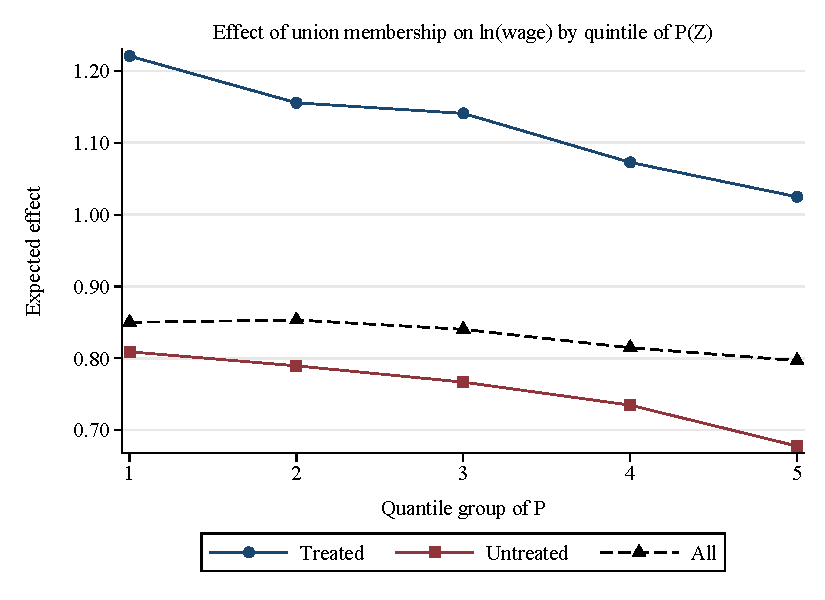
\includegraphics[width=0.48\textwidth]{fig_union3_curve.pdf}}{\fbox{\parbox{0.46\textwidth}{\centering\small \cmd{fig\_union3\_curve.pdf}\\ (from \cmd{sec7\_union3.do})}}}\hfill
\IfFileExists{fig_union3_mte.pdf}{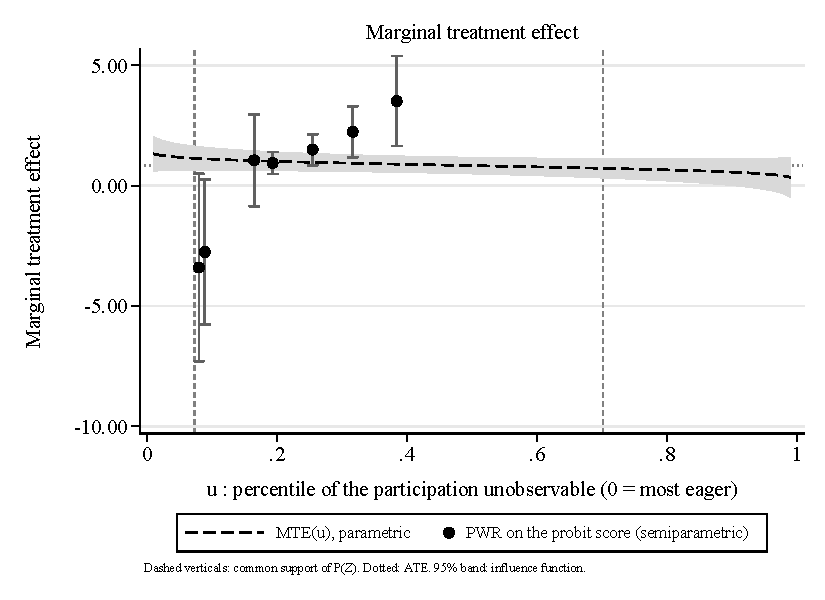
\includegraphics[width=0.48\textwidth]{fig_union3_mte.pdf}}{\fbox{\parbox{0.46\textwidth}{\centering\small \cmd{fig\_union3\_mte.pdf}\\ (from \cmd{sec7\_union3.do})}}}
\caption{\cmd{union3}, log wage, two-step route. Left: expected effect of membership by quintile of the score $P(Z)$, members, non-members and all (\cmd{esrcurve}). Right: the parametric MTE line with its 95 percent band and the semiparametric curve on the probit score (\cmd{esrmte, semipar}); dashed verticals mark the common support, the dotted line the ATE. The curve is uninformative outside the middle of the score: a single indicator instrument leaves the derivative in $P$ without variation to be estimated from (Assumption V).}
\label{fig:union3}
\end{figure}

%=======================================================================
\section{The \texorpdfstring{\cmd{esreg}}{esreg} command}\label{sec:cmd}
%=======================================================================

\subsection{What official Stata already does}\label{sec:cmd:etregress}

The model of Section~\ref{sec:model} is not new to Stata. Since
version~14, \cmd{etregress} with the option \cmd{poutcomes} fits the
``general potential-outcome model'' \citep{statacorp2025}: separate
$\sigma_j$ and $\rho_j$ by treatment group, one outcome equation in
which the treatment may be interacted with any covariate. When it is
interacted with all of them, the likelihood is~\eqref{eq:ll} and
\cmd{esreg, method(fiml)} reproduces it to every printed digit on the
samples of the manual (Section~\ref{sec:emp}); \cmd{margins,
predict(cte) subpop()} then gives the ATT, through the same formula
$\E[x(\beta_1-\beta_0)+(\rho_1\sigma_1-\rho_0\sigma_0)\lambda_1\mid D=1]$
as the expected effect of the treated in Section~\ref{sec:model:base}, where $\kappa$ appears without a name. The
control-function estimator (\cmd{cfunction}) is the stacked-moment GMM of
Section~\ref{sec:est:twostep} extended to the variance parameters; the
\cmd{twostep} option exists for the constrained model only. What the
official command does not offer is everything this paper is about:
$\kappa$ as a parameter with a standard error, its heterogeneity in $X$
and the heterogeneous regime laws, the two-step route for the general
model with its exact variance, the tests of Section~\ref{sec:tests}
(its only test is the Wald of $\rho_0=\rho_1=0$), the diagnostics of the
selection equation, the effects on the common support, the effect by
quantile, and the MTE line and curve. \cmd{movestay} \citep{lokshin2004}
fits the same likelihood with its own syntax and no post-estimation
beyond \cmd{mspredict}; \cmd{msat} \citep{araar2026msat} adds the effects,
$\kappa$, the quantile profile and the MTE after it.
Table~\ref{tab:cmds} sets the three side by side.

\begin{table}[t]
\centering
\caption{The ESR in Stata: \cmd{etregress}, \cmd{movestay}/\cmd{msat} and \cmd{esreg}}
\label{tab:cmds}
\footnotesize
\begin{tabular}{@{}L{5.0cm}L{2.1cm}L{1.6cm}L{2.1cm}L{3.3cm}@{}}
\toprule
 & \cmd{etregress} & \cmd{movestay} & \cmd{msat} & \cmd{esreg} \\
 & \cmd{poutcomes} & & (after \cmd{movestay}) & family \\
\midrule
Separate $\beta_j$, $\sigma_j$, $\rho_j$ (FIML) & interactions & yes & -- & yes \\
Two-step for the general model & -- (CF GMM) & -- & bootstrap & yes, stacked variance \\
Heterogeneous $\sigma_j$, $\rho_j$ in covariates & -- & -- & -- & \cmd{hetsigma()}, \cmd{hetrho()} \\
$\kappa=\rho_1\sigma_1-\rho_0\sigma_0$ with s.e. & -- & -- & yes & yes \\
$\kX$ and its test & -- & -- & -- & \cmd{kappa()}, \cmd{esrtest, kappa} \\
ATT, ATU, ATE with s.e. & \cmd{margins} & \cmd{mspredict} & yes & yes, plus common support \\
Effect by quantile of $P$ & -- & -- & yes & \cmd{esrcurve} \\
MTE line / semiparametric curve & -- & -- & yes & \cmd{esrmte} \\
Strength, variation, support diagnostics & -- & -- & partly & \cmd{esrdiag} \\
Specification, sufficiency, normality, pseudo-DiD tests & -- & -- & -- & \cmd{esrtest} \\
Factor variables, weights, \cmd{vce()} & yes & partly & weights & yes \\
\cmd{svy:} prefix; \cmd{svyset} weights, \cmd{hsize()} & ML only & -- & \cmd{svyset}, \cmd{hsize()} & FIML; yes \\
Test of no selection on unobservables & Wald & LR & -- & LR \\
\bottomrule
\end{tabular}
\end{table}

\subsection{The family}\label{sec:cmd:family}

The design decision was to have one estimation command and a family
of post-estimation commands, rather than one command that does
everything: each tool of Sections~\ref{sec:tests} and~\ref{sec:est}
is a command with its own syntax, its own returned results and its
own help, and the practitioner runs the ones the reading requires.
Table~\ref{tab:syntax} gives the syntax. \cmd{esreg} estimates the
model by the route chosen in \cmd{method()}, computes the effects,
$\kappa$ and their standard errors, and stores the estimation
automatically under the name \cmd{\_esreg}, and under a second name if
\cmd{store()} is given; every post-command works from \cmd{est(name)},
else from the current \cmd{e()} when it is an \cmd{esreg} estimation,
else from \cmd{\_esreg}, so that the post-commands can be run in any
order after other Stata commands have overwritten \cmd{e()}, and
several estimations can be kept and queried in one session. The
post-commands protect the user's \cmd{e()}: they hold it, re-estimate
what they need (the tests of Section~\ref{sec:tests:normal}, for
instance, refit both routes), and restore it on exit. Factor variables
and interactions are accepted everywhere; the \cmd{if}/\cmd{in}
sample and the weights of the estimation are inherited by the
post-commands through \cmd{e(sample)}, \cmd{e(wtype)} and
\cmd{e(wexp)}.

\begin{table}[!htb]
\centering
\caption{The \cmd{esreg} family: syntax}
\label{tab:syntax}
\scriptsize
\begin{tabular}{@{}L{4.2cm}L{11.2cm}@{}}
\toprule
Command & Syntax and main options \\
\midrule
estimation & \cmd{esreg} \textit{depvar} [\textit{indepvars}] [\textit{if}] [\textit{in}] [\textit{weight}]\cmd{, select(}\textit{treatvar} \cmd{=} \textit{varlist}\cmd{)} [\cmd{method(fiml}$\mid$\cmd{twostep)} \cmd{hetsigma(}\textit{varlist}\cmd{)} \cmd{hetrho(}\textit{varlist}\cmd{)} \cmd{kappa(}\textit{varlist}\cmd{)} \cmd{hermite(}\#\,[\#]\cmd{)} \cmd{vce(}\textit{vcetype}\cmd{)} \cmd{hsize(}\textit{varname}\cmd{)} \cmd{nosvyset} \cmd{store(}\textit{name}\cmd{)} \cmd{noeffects} \cmd{level(\#)} \textit{maximize options}] \\
 & \cmd{svy:} \cmd{esreg} \ldots (FIML; see Section~\ref{sec:cmd:svy}); replay: \cmd{esreg} [\cmd{, effects}] \\
predictions & \cmd{predict} \textit{newvar} [\cmd{,} \textit{statistic}]: \cmd{xb1 xb0 xbsel pr lambda1 lambda0 yc11 yc10 yc01 yc00 effect kappa rhosig1 rhosig0 sigma1 sigma0 rho1 rho0}; \cmd{predict} \textit{stub}\cmd{*, scores} \\
diagnostics & \cmd{esrdiag} [\cmd{, est(}\textit{name}\cmd{)}]: strength (LR, per-instrument $\chi^2$, pseudo-$R^2$ increment), variation ($\Var(P\mid X)/\Var(P)$, VIF of $\lambda_j$), support and extrapolated shares, effects on the common support; warnings \\
tests & \cmd{esrtest, spec} [\cmd{order(\#)} \cmd{add(}\textit{varlist}\cmd{)}] (\S\ref{sec:tests:spec}); \cmd{esrtest, suff} [\cmd{keep(}\textit{varname}\cmd{)}] (\S\ref{sec:tests:suff}); \cmd{esrtest, kappa} (\S\ref{sec:tests:kx}); \cmd{esrtest, normal} (\S\ref{sec:tests:normal}); \cmd{esrtest, pdid} [\cmd{nq(\#)} \cmd{reps(\#)}] (\S\ref{sec:tests:pdid}); all with [\cmd{est(}\textit{name}\cmd{)} \cmd{level(\#)}] \\
effect by quantile & \cmd{esrcurve} [\textit{if}] [\textit{in}]\cmd{, rank(}\textit{varname}\cmd{)} [\cmd{nq(\#)} \cmd{graph} \cmd{nose} \cmd{est(}\textit{name}\cmd{)} \cmd{saving()}] \\
marginal treatment effect & \cmd{esrmte} [\textit{if}] [\textit{in}] [\cmd{, at(}\textit{numlist}\cmd{)} \cmd{semipar} \cmd{graph} \cmd{est(}\textit{name}\cmd{)} \cmd{saving()}] \\
reading & \cmd{esrreport} [\cmd{, est(}\textit{name}\cmd{)} \cmd{nq(\#)} \cmd{lrmin(\#)} \cmd{vifmax(\#)} \cmd{extrapmax(\#)} \cmd{alpha(\#)} \cmd{export(}\textit{filename}\cmd{)} \cmd{notests}] \\
\bottomrule
\end{tabular}
\parbox{0.95\textwidth}{\footnotesize \textit{weight}: \cmd{pweight} or \cmd{iweight} (\cmd{fweight}s are refused, Section~\ref{sec:cmd:svy}). \cmd{vce()}: \cmd{oim} (default), \cmd{robust}, \cmd{cluster} \textit{clustvar}, \cmd{opg} for FIML; for the two-step, the stacked moments by observation (default), \cmd{cluster} \textit{clustvar} or \cmd{svy}. \cmd{hetsigma()}, \cmd{hetrho()} are FIML options, \cmd{kappa()} and \cmd{hermite()} two-step options (Sections~\ref{sec:model:kx} and~\ref{sec:est:augmented}). The \cmd{bootstrap} and \cmd{jackknife} prefixes apply to \cmd{esreg} as to any estimation command.}
\end{table}

\paragraph{Stored results.}
\cmd{esreg} returns \cmd{e(b)} and \cmd{e(V)} for the whole parameter
vector (FIML: the seven equations $y_1$, $y_0$, the selection
equation, $\ln\sigma_1$, $\ln\sigma_0$, $\operatorname{atanh}\rho_1$,
$\operatorname{atanh}\rho_0$; two-step: the selection equation and
the two regime blocks with their $\lambda$ terms), and organizes what
the post-commands need: the matrix \cmd{e(effects)} ($4\times5$: ATT,
ATU, ATE, $\kappa$ by estimate, standard error, parameter and sampling
variances and twice their covariance), the scalars \cmd{e(att)} \ldots
\cmd{e(se\_kappa)}, \cmd{e(sigma1)}, \cmd{e(rho1)}, \ldots,
\cmd{e(supp\_lo)}, \cmd{e(supp\_hi)}, the coefficient blocks
\cmd{e(b\_sel)}, \cmd{e(b\_1)}, \cmd{e(b\_0)}, the support and mean
Mills ratios, and the expanded variable lists \cmd{e(xvars)},
\cmd{e(zvars)}, \cmd{e(hetsigma)}, \cmd{e(hetrho)}, \cmd{e(kappavars)}.
The post-commands are \cmd{rclass}: \cmd{esrtest} returns the
statistics, degrees of freedom and $p$-values of its subtest and the
tables it prints (\cmd{r(slopes)}, \cmd{r(coefs)}, \cmd{r(link)},
\cmd{r(gamma)}, \cmd{r(q)}, \cmd{r(hermite)}, \cmd{r(strata)});
\cmd{esrdiag} its diagnostics and the flags \cmd{r(weak)},
\cmd{r(form)}; \cmd{esrcurve} the table \cmd{r(table)}; \cmd{esrmte}
the line \cmd{r(mte)} and the curve \cmd{r(mte\_sp)}; \cmd{esrreport}
the route \cmd{r(route)}, the numbered notes \cmd{r(note\#)} and the
figures they rest on.

\paragraph{The reading.}
\cmd{esrreport} runs the diagnostics and the tests on the stored
estimation and prints the four steps of Section~\ref{sec:emp}, with
notes conditioned on the results: instrument strength and form
(\cmd{lrmin()}, \cmd{vifmax()}), extrapolation (\cmd{extrapmax()}), the
sign and significance of $\kappa$ and the pattern of the pseudo-DiD
contrasts, and the route to report, decided in the order of the
assumptions---the index first (a rejected link test makes every
downstream test unreadable), then sufficiency (a rejected exclusion
biases both routes), then the conditional mean (Hermite controls: the
augmented two-step when the instrument is strong, the semiparametric
curve otherwise), then the joint law (Hausman: the two-step),
else the likelihood. The notes are statements and questions, not
verdicts; the thresholds are options, and each note names the test and
the section it rests on. \cmd{export()} writes the figures and the
notes to a plain-text sheet, the material an assistant, human or not,
can read together with the context of the study; the rules stay in
Stata, reproducible and auditable, and the interpretation stays
outside.

\subsection{Weights and survey design}\label{sec:cmd:svy}

Household surveys are the natural habitat of the model, and the family
handles their weights at every step. \cmd{esreg} accepts
\cmd{pweight}s (the probit, the regime regressions and the likelihood
are weighted, the FIML variance is then the sandwich, the two-step
variance the weighted stacked moments, the effects weighted averages)
and \cmd{iweight}s; \cmd{fweight}s are refused, since a unit of a survey
stands for its sampling weight and is not a replicated record. When no
weight is given and the
data are \cmd{svyset}, the design weight is taken by default with a
note (\cmd{nosvyset} declines it), and an explicit weight is used
alone, never on top of the \cmd{svyset} one. The option
\cmd{hsize(}\textit{varname}\cmd{)} multiplies the weight by the
household size, so that the effects are averages over individuals when
the unit of observation is the household. The post-commands inherit the
weights of the estimation.

The FIML route supports the \cmd{svy:} prefix: \cmd{esreg} declares the
\cmd{svyb}, \cmd{svyj} and \cmd{svyr} properties, accepts the
\cmd{iweight}s the prefix passes, and \cmd{predict, scores} returns
the seven equation-level scores of the likelihood, from which
\cmd{svy} builds the linearized variance for the strata, clusters and
finite-population corrections of the design---and the bootstrap,
jackknife and BRR variances of its other \cmd{vce()} options. Since
\cmd{svy} replaces \cmd{e(V)} after the command has returned, the
effects, $\kappa$ and their standard errors are recomputed from the
linearized variance the first time the estimation is replayed, or on
request with \cmd{esreg, effects}; \cmd{e(eff\_vce)} says which
variance they rest on. The two-step route does not take the prefix,
for the same reason \cmd{etregress, twostep} does not: a sequential
estimator has no single likelihood score for the prefix to linearize.
It has its own design-based variance instead, \cmd{vce(svy)}: the
influence functions of the whole procedure, aggregated through the
strata, primary units, finite-population corrections and weights of
\cmd{svyset}; \cmd{vce(cluster} \textit{clustvar}\cmd{)} sums them within
clusters. The effects follow the same aggregation by both routes, and
after \cmd{svy, subpop()} the effects, the curves and the tests are those
of the subpopulation. Under a design with weights only, the linearized
standard errors of \cmd{svy: esreg} coincide with those of \cmd{esreg}
with \cmd{pweight}s, which is one of the checks of the validation file.

\subsection{Validation and reproducibility}\label{sec:cmd:valid}

The specification of the commands is a Python reference library
(\cmd{esreg/}, about a thousand lines: likelihood and analytic score,
FIML, two-step with the stacked variance, effects, the tests and the
diagnostics), written first; every number the Stata family prints was
checked against it, value for value, on the simulated samples of this
paper, on the samples of \citet{araar2026msat}, and on the manual's
\cmd{union3} and \cmd{drugexp}. The family was also checked against the
official and community commands where they overlap: \cmd{etregress,
poutcomes} with the treatment interacted with all covariates
reproduces the FIML to the convergence tolerance and \cmd{margins,
predict(cte)} the ATT; \cmd{etregress, cfunction} reproduces the
two-step point estimates exactly and its robust variance to four
digits, which validates Proposition~\ref{prop:stacked} against an
independent implementation of the same moment conditions;
\cmd{movestay} and \cmd{msat} reproduce the likelihood and the
effects. The Monte Carlo of the tests (Section~\ref{sec:mc}) runs on the
Python library.

The standard errors were checked against oracles that do not share the
command's formulas, in a do-file with tolerances and a pass-or-fail
summary (\cmd{tests/test\_effects\_se.do}). The influence functions of
the effects, of $\kappa$, of the slope of $\kX$, of the MTE line and of
the augmented curve, by both routes and with the heterogeneous options,
equal a brute force that re-runs the whole estimation with the weight of
one observation moved (slope of one within $5\times10^{-5}$ for the
two-step and the convergence tolerance of \cmd{ml} for the likelihood);
aggregated by cluster they give \cmd{ml}'s \cmd{vce(cluster)}, and through
the design the \cmd{svy} prefix's linearized variance; the pseudo-DiD
equals an independent implementation in the reference library to
$10^{-6}$ and the bootstrap of its whole procedure within a few percent
on continuous indices. The Monte Carlo of the standard errors closing
Section~\ref{sec:mc} and of the augmented two-step
(Section~\ref{sec:est:augmented}) runs in Stata, from the do-files of the
\cmd{tests/mc} folder.

The commands and the replication material of the paper share one
repository, \url{https://github.com/aabbdd12/esreg}. The package is
installed from Stata with
\begin{quote}
\footnotesize\cmd{. net install esreg, from("https://raw.githubusercontent.com/aabbdd12/esreg/v1.0.0/") replace}\\
\cmd{. net get esreg, from("https://raw.githubusercontent.com/aabbdd12/esreg/v1.0.0/") replace}
\end{quote}
(the second line copies the data of the examples of \cmd{help esreg};
replacing \cmd{v1.0.0} by \cmd{main} installs the latest version): the ado
files, the help files with their clickable examples and the dialog box; it
will also be submitted to the SSC archive. The folder \cmd{replication} of
the repository, which the installation does not copy
(\url{https://github.com/aabbdd12/esreg/tree/v1.0.0/replication}), holds
the Python library and the Monte Carlo scripts with their outputs, the
simulated samples with their generating scripts and seeds, the Stata
do-files and logs that produce every table and figure, including
Section~\ref{sec:emp}, the raw results of the Monte Carlo of the standard
errors and of the brute force, and the \LaTeX\ source; the paths quoted in
this paper are relative to it. A user who wants the command does not
download the paper's experiments, and a reader who wants to check a table
finds it reproduced by one script, in Python and in Stata, from the same
data. The package
installed from the repository reproduces, on the \cmd{union3} sample,
every number of Section~\ref{sec:emp} to the last printed digit.

%=======================================================================
\section{Conclusion}\label{sec:concl}
%=======================================================================

The endogenous switching regression is fragile in the places where its
selection equation is asked to do too much, and robust elsewhere; the
purpose of this paper was to say where those places are and to give
the practitioner a test for each. Ordered by what they cost, the
assumptions are a correctly specified normal index, instruments that
act only through it, enough variation in it, a linear conditional mean
of the regime errors, and normality around that mean. The first three
are properties of the selection equation and are tested on the probit
and the two regime regressions; the fourth is tested by Hermite
controls, which, kept in the estimation when it fails, give the
augmented two-step at a price in precision; the fifth by a Hausman
contrast between the two routes, and
it is the only one that can be dropped without loss, since the two-step
route does not need it. The pseudo-DiD on the index closes the circle
by reading selection on gains off a two-by-two table with the linear
conditional mean alone, and the extension to $\kappa(x)$ turns the
heterogeneity of that selection into a hypothesis.

Three lessons come out of the experiments and the example. The tests
have their size and do not confound each other: the sufficiency test is
flat under a nonlinear conditional mean, the Hermite test is flat under
skewed errors, the link test is flat under both, and the contrast
between the routes is the one statistic that answers to two things,
with its neighbours saying which. The likelihood, when its joint law is
wrong, returns a confident wrong number---the manual example's ATE in
dollars---and the two-step, which needs less, returns a less confident
one, right if the exclusion of the instrument holds; the standard error
of the two-step, computed exactly from the stacked moments, is the honest
measure of what a single indicator instrument can bear, and on the
manual's data that exclusion is what no test can check. And the semiparametric tier, which needs the least,
also needs the most from the data: without variation in the score it has
nothing to work with, and on data like the manual's the parametric line
is all there is, which is why its assumptions must be tested rather than
assumed.

Three things are left for later work. The copula tier of
Section~\ref{sec:est:copula}, which replaces trivariate normality by a
family of joint laws and reports the untreated effect as a band across
them, is described but not implemented; it is the practicable
counterpart of the bounds of \citet{mogstad2018} inside the parametric
model. The exclusion of the instrument held out by the sufficiency test
is the one assumption no test of the family checks
(Section~\ref{sec:tests:suff}), and a sensitivity analysis to a direct
effect of that instrument would give it a reading. And a second
empirical application, on a household survey with
two instruments and a program with a clear selection on gains, would
show the toolkit where it was designed to work; the manual example
shows it where it is needed. The commands, their Python reference
implementation and the replication material of every table and figure
are available with the paper (\url{https://github.com/aabbdd12/esreg}).

\appendix
%=======================================================================
\section{Proofs}\label{app:proofs}
%=======================================================================

Propositions~\ref{prop:kx} and~\ref{prop:suff} are proved in the text.
Throughout, $v=Z\gamma$, $\lambda_1(v)=\phi(v)/\Phi(v)$,
$\lambda_0(v)=\phi(v)/\Phi(-v)$, and for $u\sim N(0,1)$ the truncated
moments are
\begin{equation}\label{eq:trunc}
\begin{aligned}
\E[u\mid u>-v]&=\lambda_1(v), & \E[u^2\mid u>-v]&=1-v\lambda_1(v), & \E[u^3\mid u>-v]&=(v^2+2)\lambda_1(v),\\
\E[u\mid u<-v]&=-\lambda_0(v), & \E[u^2\mid u<-v]&=1+v\lambda_0(v), & \E[u^3\mid u<-v]&=-(v^2+2)\lambda_0(v),
\end{aligned}
\end{equation}
which follow from $\int_a^\infty u^k\phi(u)\,du$ by integration by parts
($\phi'(u)=-u\phi(u)$): $\int_a^\infty u\phi=\phi(a)$,
$\int_a^\infty u^2\phi=a\phi(a)+1-\Phi(a)$,
$\int_a^\infty u^3\phi=(a^2+2)\phi(a)$, evaluated at $a=-v$ and divided
by $\Phi(v)$; the lower tail follows by symmetry.

\subsection{Proposition~\ref{prop:routes} (identification by route)}

\emph{(i)} Under A1--A3, $(Y,D)$ given $Z$ has the density
\eqref{eq:ll}, the standard switching-regression likelihood of
\citet[p.~224]{maddala1983}. Identification of $\gamma$ comes from the
marginal probit $P(D=1\mid Z)=\Phi(Z\gamma)$ under E and V (a column of
$Z$ outside $X$ with non-zero coefficient rules out that $Z\gamma$ is a
function of $X$ alone, and the constant is identified by the normalization
$\Var(u)=1$). Given $\gamma$, the conditional density of $Y$ given
$D=1,X,Z$ is that of $X\beta_1+\omega_1$ given $u>-Z\gamma$, a normal
truncated through its correlation with $u$; its mean
$X\beta_1+\rho_1\sigma_1\lambda_1(v)$ and variance
$\sigma_1^2\{1-\rho_1^2\lambda_1(v)(\lambda_1(v)+v)\}$ vary with $v$ at
fixed $X$ by V, so that $\beta_1$, $\rho_1\sigma_1$ and then $\sigma_1^2$
and $\rho_1^2$ are identified from the first two conditional moments, and
the sign of $\rho_1$ from the first; the untreated regime is symmetric.
The parameters identify $\kappa=\rho_1\sigma_1-\rho_0\sigma_0$, the
effects and the line \eqref{eq:mte} at every $p\in(0,1)$, since the line
is a function of the parameters alone.

\emph{(ii)} Under A1--A2 only the conditional means are specified:
$\E[Y\mid X,Z,D=1]=X\beta_1+\rho_1\sigma_1\lambda_1(v)$ and
$\E[Y\mid X,Z,D=0]=X\beta_0-\rho_0\sigma_0\lambda_0(v)$, which is
Proposition~\ref{prop:kx} with $W=1$; $\gamma$ is identified by the
probit as in (i). The products $\rho_j\sigma_j$ are identified, hence
$\kappa$, the effects and the line \eqref{eq:mte}, which depend on the
parameters only through $\beta_1-\beta_0$, $\kappa$ and $\gamma$. The
conditional variance is not specified under A2, so $\sigma_j$ and
$\rho_j$ are not separately identified; the residual variance of the
regime regression identifies $\sigma_j^2$ only under the normal
truncation formula, that is under A3. The line is a parametric
extrapolation outside the support of $P(Z)$, where no conditional mean
is observed: on the support it is the identified function
$\E[Y\mid X,P,D=j]$ evaluated under A2, outside it is the assumption.

\emph{(iii)} Under A1 alone, with $v$ the single index, $P=\Phi(v)$ is
identified and $(X,P)$ carries the same information as $(X,v)$. By
\citet[Theorem~1]{heckman2005}, when $D=\1\{P>U\}$ with $U$ uniform and
independent of $Z$ given $X$ (here $U=\Phi(-u)$, and independence of
$u$ from $Z$ given $X$ is A1 with S), the marginal treatment effect
$\MTE(x,p)=\E[Y_1-Y_0\mid X=x,U=p]$ equals $\partial\E[Y\mid X=x,P=p]/\partial p$
at every $p$ in the support of $P$ given $X=x$, and
$m_j(x,p)=\E[Y_j\mid X=x,P=p,D=j]$ are identified there as the observed
conditional means. No functional form is used, so nothing is identified
outside the support. If A2 holds in addition, $\E[Y_1-Y_0\mid X,U=p]$ is
affine in $\Phi^{-1}(1-p)$ with slope $-\kappa$ and $\kappa$ is the
common slope; if the conditional mean is not linear in $u$ the slope
varies with $p$ and no single number is the slope. \hfill$\square$

\subsection{Proposition~\ref{prop:normal} (separation of the two tests)}

\emph{The Hermite terms.} Let $\E[\omega_j\mid u]=\sum_{k\ge1}a_{jk}H_k(u)$
with $H_1(u)=u$, $H_2(u)=u^2-1$, $H_3(u)=u^3-3u$ the probabilists'
Hermite polynomials, and let S hold so that $\E[\omega_j\mid X,Z,u]=\E[\omega_j\mid u]$.
Then $\E[\omega_1\mid X,Z,D=1]=\sum_k a_{1k}\E[H_k(u)\mid u>-v]$, and by
\eqref{eq:trunc}, $\E[H_1\mid u>-v]=\lambda_1$,
$\E[H_2\mid u>-v]=-v\lambda_1$,
$\E[H_3\mid u>-v]=(v^2+2)\lambda_1-3\lambda_1=(v^2-1)\lambda_1$; below the
threshold, $\E[H_1\mid u<-v]=-\lambda_0$, $\E[H_2\mid u<-v]=v\lambda_0$,
$\E[H_3\mid u<-v]=-(v^2-1)\lambda_0$. This is \eqref{eq:hermite}. Under
A2, $a_{j2}=a_{j3}=0$ whatever the law of $\omega_j$ given $u$ beyond
its conditional mean: a skewed $\omega_j$ with $\E[\omega_j\mid u]$ linear
in $u$ has zero Hermite coefficients, so the population regression of $Y$
on $X$, $\lambda_j$ and the two Hermite controls in regime $j$ has zero
coefficients on the controls, and the Wald statistic built on the stacked
variance of Proposition~\ref{prop:stacked} (which needs A1--A2 and
finite fourth moments, not A3) is asymptotically $\chi^2(4)$. Under a
failure of A2 with $a_{j2}$ or $a_{j3}$ non-zero, the population
coefficients are non-zero and the statistic diverges; the regression on
$X$ and $\lambda_j$ alone then omits a regressor correlated with
$\lambda_j$, so its coefficient on $\lambda_j$ converges to
$\rho_j\sigma_j$ plus the omitted-variable term, and the likelihood, whose
conditional mean is $X\beta_j\pm\rho_j\sigma_j\lambda_j$, is misspecified
in the same direction: both routes are inconsistent for
$\rho_j\sigma_j$ and $\kappa$, and neither line is the MTE.

\emph{The Hausman contrast.} Let $q$ be the common parameter and
$\hat q_{2S}$, $\hat q_F$ the two estimators. Under A1--A3, both are
regular $\sqrt n$-consistent estimators with influence functions
$\psi_{2S,i}$ and $\psi_{F,i}$ (the two-step from Proposition~%
\ref{prop:stacked} mapped to $q$, the likelihood from the information
equality, mapped to $q$ by the delta method for
$\rho_j\sigma_j=\tanh(c_j)\exp(a_j)$), so that
$\sqrt n(\hat q_{2S}-\hat q_F)=n^{-1/2}\sum_i(\psi_{2S,i}-\psi_{F,i})+o_p(1)\to N(0,\Omega_\Delta)$
with $\Omega_\Delta=\E[(\psi_{2S}-\psi_F)(\psi_{2S}-\psi_F)']$; the
estimator \eqref{eq:hausman} replaces $\psi$ by its sample version
evaluated at the estimates and is consistent for $\Omega_\Delta$ by the
law of large numbers and the continuity of $\psi$ in the parameters. If
$\Omega_\Delta$ has rank $r$, the quadratic form with the
Moore--Penrose inverse converges to $\chi^2(r)$, and $\hat V_\Delta^+$
with the estimated rank converges to it too. Since the likelihood is
efficient under A1--A3, $\E[\psi_{2S}\psi_F']=\E[\psi_F\psi_F']$
\citep[the lemma of][]{hausman1978}, and $\Omega_\Delta=V_{2S}-V_F$, the
usual Hausman covariance; \eqref{eq:hausman} is positive semi-definite
in every sample while the difference of the two estimated variances need
not be. Under a failure of A3 that keeps A1--A2, the two-step remains
consistent for $q$ (Proposition~\ref{prop:kx} with $W=1$ uses the
conditional mean only) while the likelihood converges to the
pseudo-true value that minimizes the Kullback--Leibler distance to the
normal density, which differs from $q$ unless the true regime
distributions are normal (the truncation formula that the likelihood
applies to the observed regime is then wrong at every $v$, and the
maximizer trades the fit of the mean against the fit of the shape); the
difference converges to a non-zero vector and the statistic diverges,
while \eqref{eq:hausman} remains a consistent estimator of the
variance of the difference of two $\sqrt n$-consistent estimators of
different limits, so that the contrast is reported with a valid
standard error. \hfill$\square$

\subsection{Proposition~\ref{prop:pdid} (pseudo-DiD)}

\emph{First part.} Under A1--A2, E and V, for a treated unit in stratum
$s$ of $v$, $\E[Y\mid X,v,D=1]=X\beta_1+\rho_1\sigma_1\lambda_1(v)$ by
\eqref{eq:trunc}. In the within-treated regression of $Y$ on $X$ and the
indicator $T$ of the top stratum over the units of the top and bottom
strata, $X\beta_1$ is fitted exactly by the regressors, so that the
population coefficient of $T$ is $\rho_1\sigma_1$ times the coefficient
of $T$ in the same regression of $\lambda_1(v)$, which is $\pi_1$:
$C_1=\rho_1\sigma_1\pi_1$, with no approximation. The untreated regression
gives $C_0=-\rho_0\sigma_0\pi_0$ in the same way from
$\E[Y\mid X,v,D=0]=X\beta_0-\rho_0\sigma_0\lambda_0(v)$. Since $\hat\gamma$
and the sample quantiles that cut the strata are consistent, the sample
contrasts converge to their population values; $\pi_1$ and $\pi_0$ are
non-zero by V and the strict monotonicity of $\lambda_j$ as long as the
adjustment for $X$ does not undo the ordering of the strata, which the
command shows by reporting them. Hence $C_1/\pi_1\to\rho_1\sigma_1$,
$C_0/\pi_0\to-\rho_0\sigma_0$ and
$\hat\kappa_{DD}\to\rho_1\sigma_1-\rho_0\sigma_0=\kappa$ for any fixed
$G\ge2$. The estimating equations of the whole procedure (probit score,
quantile conditions of the cut points, the regressions) are just
identified, and the influence function $-J^{-1}m_i$ is the M-estimation
result used for Proposition~\ref{prop:stacked}, the indicators of the
strata being smoothed for the derivatives in $\gamma$ and in the cut
points.

\emph{Second part.} Under A2 alone with $u$ continuous and any law $F_u$,
$\E[\omega_1\mid X,v,D=1]=\rho_1\sigma_1\,m_1(v)$ with
$m_1(v)=\E[u\mid u>-v]$, and $\E[\omega_0\mid X,v,D=0]=\rho_0\sigma_0\,m_0(v)$
with $m_0(v)=\E[u\mid u<-v]$. Both $m_1$ and $m_0$ are strictly decreasing
in $v$: raising $v$ lowers the threshold $-v$, which adds units with
smaller $u$ to the upper tail and removes units with the largest $u$ of
the lower tail, so that the conditional mean falls in both (formally,
$\partial m_1/\partial v=-f_u(-v)\{m_1(v)+v\}/\{1-F_u(-v)\}<0$ since
$m_1(v)>-v$, and symmetrically for $m_0$). Hence in the population
$C_1=\rho_1\sigma_1\pi^m_1$ and $C_0=\rho_0\sigma_0\pi^m_0$, with $\pi^m_j$
the $X$-adjusted contrasts of $m_j(v)$, negative when the adjustment for
$X$ preserves the ordering of the two strata; in the normal case
$m_1=\lambda_1$ and $m_0=-\lambda_0$, so that $\pi^m_1=\pi_1$ and
$\pi^m_0=-\pi_0$, and in general the sign of $C_1$ is that of
$-\rho_1\sigma_1$ and the sign of $C_0$ that of $-\rho_0\sigma_0$. The
signs need neither the normality of $u$ (A1) nor the joint law (A3), only
the monotonicity of a truncated mean. \hfill$\square$

\subsection{Proposition~\ref{prop:stacked} (variance of the two-step estimator)}

Write $\vartheta=(\gamma',\beta_1',\theta_1',\beta_0',\theta_0')'$ and let
$g_i(\vartheta)$ be the stacked moment \eqref{eq:moments}. The two-step
estimator solves $\sum_ig_i(\hat\vartheta)=0$ exactly: the first block is
the probit first-order condition, solved by $\hat\gamma$ alone; the
second and third blocks are the normal equations of the regime
regressions given $\hat\gamma$, solved by
$(\hat\beta_j,\hat\theta_j)$. It is therefore the exactly identified
GMM (M-) estimator with moment function $g_i$. Under A1--A2, E, S and V,
$\E[g_i(\vartheta_0)]=0$: the probit score has mean zero at the true
$\gamma$ under A1; the regime moments have mean zero because
$\E[Y-r_{ji}(\beta_j',\theta_j')'\mid X,Z,D=j]=0$ under A1--A2 with S
(the conditional mean is exactly $r_{ji}'(\beta_j',\theta_j')'$ and $r_{ji}$
is a function of $(X,Z)$). The Jacobian $G=\E[\partial g_i/\partial\vartheta']$
is block lower-triangular, with $\E[\partial s_i/\partial\gamma']$ (the
negative probit information) in the first block, $-\E[D_ir_{1i}r_{1i}']$
and $-\E[(1-D_i)r_{0i}r_{0i}']$ on the diagonal of the regime blocks,
and the off-diagonal blocks
$\E[D_i\,\partial\{r_{1i}'(y_i-r_{1i}(\beta_1',\theta_1')')\}/\partial\gamma']$,
which carry $\partial\lambda_1(z_i\gamma)/\partial\gamma'=-\lambda_1(\lambda_1+z_i\gamma)z_i$
and its mirror for $\lambda_0$; $G$ is nonsingular by the identification
of $\gamma$ and the rank conditions of Proposition~\ref{prop:kx}
(nonsingular $\E[r_{ji}r_{ji}'\mid D=j]$). With $\Omega=\E[g_ig_i']$
finite (finite fourth moments of the regime errors and of $r_{ji}$),
the standard M-estimation expansion
$0=n^{-1/2}\sum_ig_i(\vartheta_0)+G\sqrt n(\hat\vartheta-\vartheta_0)+o_p(1)$
\citep[Theorem~12.3]{wooldridge2010} gives
$\sqrt n(\hat\vartheta-\vartheta_0)\to N(0,G^{-1}\Omega G^{-1\prime})$,
and \eqref{eq:stacked} is consistent by the law of large numbers applied
to $\hat G$ (the analytic or numerical derivative evaluated at
$\hat\vartheta$) and to $\sum_ig_ig_i'/n$. Because the off-diagonal blocks
of $G$ are not zero, $G^{-1}$ propagates the sampling error of
$\hat\gamma$ into the regime blocks: this is the first-step correction of
\citet{newey1984}, and setting these blocks to zero gives the
regression-by-regime variance that ignores it. Because $\Omega$ is the
outer product of the moments, the regime blocks of the variance are of
the heteroskedasticity-robust form, which is what the truncation induces
($\Var(Y\mid X,Z,D=j)$ depends on $v$ under A3, and is unrestricted
under A2). Finally $\kappa=\theta_1-\theta_0$ and $\kX=W'(\theta_1-\theta_0)$
are continuously differentiable functions of $\vartheta$, so the delta
method applies to $\hat V$. An effect is in addition an average over the
units: expanding $\hat\tau=\sum_iw_i\tau_i(\hat\vartheta)/\sum_iw_i$ in
$\hat\vartheta$ and in the empirical distribution gives
$\hat\tau-\tau=\sum_i\phi_i+o_p(n^{-1/2})$ with $\phi_i$ of
\eqref{eq:if:effects}, whose first term is the parameter part and second
the sampling part; both depend on $(D_i,Z_i)$, so that the variance
$\sum_i\phi_i^2$ keeps their covariance. \hfill$\square$

%=======================================================================
\section{Monte Carlo design}\label{app:dgp}
%=======================================================================

\paragraph{Baseline.} $x,z,u\sim N(0,1)$ independent;
$D=\1\{0.2+0.3x+0.9z+u>0\}$; $Y_1=1.0+1.2x+\omega_1$,
$Y_0=0.5+0.4x+\omega_0$, $\omega_1=0.78u+\varepsilon_1$ with
$\Var(\varepsilon_1)=1.3^2-0.78^2$, $\omega_0=-0.30u+\varepsilon_0$ with
$\Var(\varepsilon_0)=1-0.09$, so that $\sigma_1=1.3$, $\sigma_0=1$,
$\rho_1=0.6$, $\rho_0=-0.3$, $\kappa=1.08$. The designs N, H, C1, C2 of
\citet[Appendix B]{araar2026sog} are used as such (\cmd{mc\_common.py});
H sets $\beta_1=(2.5,0.4)$ and $\omega_1=\omega_0=0.5u+\varepsilon$; C1
keeps $\omega_0=-0.30u+0.95\varepsilon_0$ and sets
$\omega_1=\omega_0+\kappa\{u+0.5\,(u^3-3u)\}+0.8\varepsilon_1$, so that the
gain is cubic in $u$ with linear part $\kappa$; C2 draws $\varepsilon_j$
from a centred log-normal with skewness parameter $0.5$.

\paragraph{Switches of this paper.}
Q: $D=\1\{0.2+0.3x+0.9z+0.5(z^2-1)+u>0\}$ with the baseline outcomes, the
working probit on $(x,z)$ (\cmd{mc\_spec.py}).
K: $\omega_1=(0.78+s\,x)u+\varepsilon_1$, so that $\kX=1.08+s\,x$
(\cmd{mc\_kappa\_x.py}). S, Z, DH, U3: two instruments,
$D=\1\{0.2+0.3x+0.7z_1+0.6z_2+u>0\}$; Z adds $-0.3z_2$ to both potential
outcomes; DH replaces the selection by
$D=\1\{0.3+0.3x+0.9z_1+e_1>0\}\cdot\1\{0.6+0.3x+0.9z_2+e_2>0\}$ with
$\omega_j$ tied to $e_1$; U3 adds $0.6\,(u^3-3u)/\sqrt6$ to $\omega_1$
(\cmd{mc\_sufficiency.py}). Strength: $\gamma_z\in\{0.9,0.45,0.2,0\}$
(\cmd{mc\_strength.py}). Normality: N, C2, C1 (\cmd{mc\_normal.py}).
Standard errors (end of Section~\ref{sec:mc}): N by both routes and K by
the two-step, $n=2{,}000$, in Stata (\cmd{tests/mc/mc\_se.do}); the
augmented two-step (Section~\ref{sec:est:augmented}): N and C1,
$n=2{,}000$, the line and the augmented routes on the same samples
(\cmd{tests/mc/mc\_aug.do}). Seeds are fixed in every script; the single-sample validation files \cmd{esr\_link}, \cmd{esr\_kx},
\cmd{esr\_suff}, \cmd{esr\_dh} are the draws with seed 2026 of Q, K
($s=0.4$), S and DH.
All scripts, the Python reference library and the Stata do-files that
reproduce the tables are in the folder \cmd{replication} of the
repository (Section~\ref{sec:cmd:valid}).

%=======================================================================
\begin{thebibliography}{99}\small

\bibitem[Araar(2026a)]{araar2026sog} Araar, A. (2026). Estimating treatment
effects under selection on gains: models, assumptions, and policy
implications. Zenodo, \url{https://doi.org/10.5281/zenodo.22672713}.

\bibitem[Araar(2026b)]{araar2026msat} Araar, A. (2026). Treatment effects after
endogenous switching regression: the \cmd{msat} postestimation command. PEP
technical note, Zenodo, \url{https://doi.org/10.5281/zenodo.22673090}.

\bibitem[Araar(2026c)]{araar2026pwr} Araar, A. (2026). Exploring heterogeneous
effects: quantile models and percentile weights regression. Zenodo,
\url{https://doi.org/10.5281/zenodo.20315684}.

\bibitem[Andresen(2018)]{andresen2018} Andresen, M. E. (2018). Exploring
marginal treatment effects: Flexible estimation using Stata. \textit{Stata
Journal}, 18(1), 118--158.

\bibitem[Brave and Walstrum(2014)]{brave2014} Brave, S., \& Walstrum, T.
(2014). Estimating marginal treatment effects using parametric and
semiparametric methods. \textit{Stata Journal}, 14(1), 191--217.

\bibitem[Brinch et al.(2017)]{brinch2017} Brinch, C. N., Mogstad, M., \&
Wiswall, M. (2017). Beyond LATE with a discrete instrument. \textit{Journal
of Political Economy}, 125(4), 985--1039.

\bibitem[Pregibon(1980)]{pregibon1980} Pregibon, D. (1980). Goodness of link
tests for generalized linear models. \textit{Applied Statistics}, 29(1),
15--24.

\bibitem[Cornelissen et al.(2016)]{cornelissen2016} Cornelissen, T.,
Dustmann, C., Raute, A., \& Sch\"onberg, U. (2016). From LATE to MTE:
Alternative methods for the evaluation of policy interventions.
\textit{Labour Economics}, 41, 47--60.

\bibitem[Hausman(1978)]{hausman1978} Hausman, J. A. (1978). Specification
tests in econometrics. \textit{Econometrica}, 46(6), 1251--1271.

\bibitem[Heckman(1976)]{heckman1976} Heckman, J. J. (1976). The common
structure of statistical models of truncation, sample selection and limited
dependent variables and a simple estimator for such models. \textit{Annals
of Economic and Social Measurement}, 5(4), 475--492.

\bibitem[Heckman(1978)]{heckman1978} Heckman, J. J. (1978). Dummy endogenous
variables in a simultaneous equation system. \textit{Econometrica}, 46(4),
931--959.

\bibitem[Maddala(1983)]{maddala1983} Maddala, G. S. (1983).
\textit{Limited-Dependent and Qualitative Variables in Econometrics}.
Cambridge: Cambridge University Press.

\bibitem[Newey(1984)]{newey1984} Newey, W. K. (1984). A method of moments
interpretation of sequential estimators. \textit{Economics Letters}, 14(2--3),
201--206.

\bibitem[Roy(1951)]{roy1951} Roy, A. D. (1951). Some thoughts on the
distribution of earnings. \textit{Oxford Economic Papers}, 3(2), 135--146.

\bibitem[Heckman and Vytlacil(2005)]{heckman2005} Heckman, J. J., \&
Vytlacil, E. (2005). Structural equations, treatment effects, and econometric
policy evaluation. \textit{Econometrica}, 73(3), 669--738.

\bibitem[Lokshin and Sajaia(2004)]{lokshin2004} Lokshin, M., \& Sajaia, Z.
(2004). Maximum likelihood estimation of endogenous switching regression
models. \textit{Stata Journal}, 4(3), 282--289.

\bibitem[Mogstad et al.(2018)]{mogstad2018} Mogstad, M., Santos, A., \&
Torgovitsky, A. (2018). Using instrumental variables for inference about
policy relevant treatment parameters. \textit{Econometrica}, 86(5),
1589--1619.

\bibitem[StataCorp(2025)]{statacorp2025} StataCorp (2025). \textit{Stata 19
Causal Inference and Treatment-Effects Estimation Reference Manual}. College
Station, TX: Stata Press. Entry \cmd{etregress}.

\bibitem[Vella and Verbeek(1998)]{vella1998} Vella, F., \& Verbeek, M. (1998).
Whose wages do unions raise? A dynamic model of unionism and wage rate
determination for young men. \textit{Journal of Applied Econometrics},
13(2), 163--183.

\bibitem[Wooldridge(2010)]{wooldridge2010} Wooldridge, J. M. (2010).
\textit{Econometric Analysis of Cross Section and Panel Data}, 2nd ed.
Cambridge, MA: MIT Press.

\end{thebibliography}

\end{document}
